       \documentclass[12pt,pdftex,letterpaper]{article}
            \usepackage{setspace}
            \usepackage[dvips,]{graphicx} %draft option suppresses graphics dvi display
%            \usepackage{lscape}
%            \usepackage{latexsym}
%            \usepackage{endnotes}
%            \usepackage{epsfig}
%           \singlespace
            \setlength{\textwidth}{6.5in}
            \setlength{\textheight}{9in}
            \addtolength{\topmargin}{-\topmargin} 
            \setlength{\oddsidemargin}{0in}
            \setlength{\evensidemargin}{0in}
            \addtolength{\headsep}{-\headsep}
            \addtolength{\topskip}{-\topskip}
            \addtolength{\headheight}{-\headheight}
            \setcounter{secnumdepth}{2}
%            \renewcommand{\thesection}{\arabic{section}}
            % \renewcommand{\footnote}{\endnote}
            \newtheorem{proposition}{Proposition}
            \newtheorem{definition}{Definition}
            \newtheorem{lemma}{lemma}
            \newtheorem{corollary}{Corollary}
            \newtheorem{assumption}{Assumption}
            \newcommand{\Prob}{\operatorname{Prob}}
            \clubpenalty 5000
            \widowpenalty 5000
            \renewcommand{\baselinestretch}{1.35}
            
            \usepackage{amsmath}
            \usepackage{amsthm}
            \usepackage{amsfonts}
            \usepackage{amssymb}
            \usepackage{bbm}
            \usepackage{float}
            \usepackage{graphicx}
            \usepackage{multirow}
            \usepackage{natbib}
            \usepackage{longtable}
            \usepackage{subcaption}
            \usepackage{enumerate}
            \usepackage{setspace}
            \usepackage{cancel}
            \usepackage{hyperref}
%            \usepackage[nofiglist, notablist, nomarkers]{endfloat}
            \usepackage{xr}
            \externaldocument{HiddenHealth}
            
            \newcommand{\der}[2]{\frac{\text{d}#1}{\text{d}#2}}
            \newcommand{\pd}[2]{\frac{\partial#1}{\partial#2}}
            \newcommand{\E}{\operatorname{E}}
            \newcommand{\N}{\mathbb{N}}
            \newcommand{\R}{\mathbb{R}}
            
            \newcommand{\Health}{h}
			\newcommand{\ExpHealth}{\overline{\Health}}
			\newcommand{\TopHealth}{H}
			\newcommand{\Report}{x}
			\newcommand{\Age}{j}
			\newcommand{\Sex}{s}
			\newcommand{\AgeMin}{\underline{\Age}}
			\newcommand{\AgeMax}{\overline{\Age}}
			\newcommand{\AgeIncr}{\hat{\Age}}
			\newcommand{\Corr}{\rho}
			\newcommand{\HealthInitMean}{\mu_0}
			\newcommand{\HealthInitStd}{\sigma_0}
			\newcommand{\Cut}{\chi}
			\newcommand{\DiscreteCut}{\zeta}
			\newcommand{\MortParam}{\theta}
			\newcommand{\CorrParam}{\gamma}
			\newcommand{\HealthParam}{\beta}
			\newcommand{\LatentParam}{\alpha}
			\newcommand{\HealthShock}{\epsilon}
			\newcommand{\ShockMean}{\mu}
			\newcommand{\ShockStd}{\sigma}
			\newcommand{\MixProb}{q}
			\newcommand{\ReportShock}{\eta}
			\newcommand{\TypeProb}{p}
			\newcommand{\TypeProbPcvd}{\widetilde{\TypeProb}}
			\newcommand{\ReportStd}{\varsigma}
			\newcommand{\Data}{X}
			\newcommand{\ParamVec}{\Delta}
			\newcommand{\LivPrb}{\Omega}
			\newcommand{\CumLivPrb}{\omega}
			\newcommand{\TransPrb}{\Xi}
			\newcommand{\HealthDstn}{\Lambda}
			\newcommand{\ReportPrb}{\Psi}
			\newcommand{\HealthDstnPcvd}{\widetilde{\Lambda}}
			\newcommand{\LL}{\pi}
			\newcommand{\RootDir}{..}
			\newcommand{\FigsDir}{\RootDir/Figures}
			\newcommand{\TablesDir}{\RootDir/Tables}
           
						
\begin{document}

\setcounter{table}{3}

\setcounter{figure}{10}

\setcounter{equation}{7}

\appendix

\section*{Online Appendix}

Appendix~\ref{app:LitQuotes} expands on the discussion in Section~\ref{sec:StructuralSRHS} to provide more detailed references to how SRHS has been used to estimate or calibrate health dynamics in structural models. Appendix~\ref{app:Estimation} provides details on the numeric methods used to compute the log likelihood function for the latent health model, which were only summarized in Section~\ref{sec:Estimation}. Appendix~\ref{app:MoreSpecs} presents additional specifications of the latent health model, including on the HRS, PSID, and MEPS data independently as well as a simplified model that drops two key features. Appendix~\ref{app:MoreFigs} provides many more figures related to those in the main paper, but were excluded for length and space considerations.


\section{Prior Structural Work Using SRHS}\label{app:LitQuotes}

This appendix provides a review of papers with a dynamic structural model that includes individual health as a state variable.  Its sole intent is to demonstrate that the ``simple dynamics'' of health described in Section \ref{sec:Intro} are employed nearly universally, often without much elaboration or justification; relevant quotations are offered when possible.  Most of these works were published in the past decade or so, with some exceptions.

The first known (to me) dynamic structural model to include health as a state variable is found in \cite{RustPhelan97}, who use data from the Retirement History Survey, the precursor to the HRS, to explore how Social Security and Medicare rules motivate retirement behavior in an incomplete markets model.  They model the health state of a living individual as binary, with bad health indicated by answering affirmatively to either of, ``Do you have a health condition, physical handicap, or disability that limits how well you get around?'' or, ``Does your health limit the kind or amount of work or housework you can do?'' (p799-800).  The authors segregate ``the Markov transition matrix...\ representing individuals' \textit{one step ahead} beliefs'' into five components, one for each discrete state dimension.  These are each estimated separately in the first stage of their structural estimation; specifically, ``The marital status, health status, and mortality probabilities...\ were specified as binary logit probabilities and estimated via maximum likelihood.''  Although not stated directly, these quotes seem to imply that the estimation was conducted using only one-period transitions.

Two papers by the same coauthor team use HRS data to estimate transition probabilities of a binary health state.  \cite{BlauGilleskie06} estimate a structural model of joint decision-making by older married couples in which, ``[t]he transition probabilities are specified as first-order Markov logit processes.'' (p940)  In an early example of the now-standard approach, the authors use SRHS as the sole empirical measure of health, and combine the top three categories and bottom two categories to define their binary health state.  The authors write that, ``We take...\ health transitions from $t=$1-2, 2-3, and 3-4 as quantities to be explained by the model.  The model is estimated by maximum likelihood. The likelihood contribution is the product of [other outcome probabilities] and health transition probabilities.'' (p944)  The health process in \cite{BlauGilleskie08} is more complicated, but the same binary definition of health is used (p490).  They write, ``The health state in periods $t+1$ is determined by health in $t$, the medical care choices during period $t$, age, permanent unobserved heterogeneity, and an i.i.d.\ shock.'' (p482)  The transition probability is modeled as a logit with death as a third possible outcome, and the estimation is by maximum likelihood.  In both papers, an individual's reported health status is taken as given, so all transitions between binary states are treated as if they represent a true change in health.

\cite{Khwaja10} presents another dynamic discrete choice model estimated by maximum likelihood using HRS data.  Khwaja maintains all five categories of SRHS, and allows transition probabilities to be affected by the individual's discrete decisions over smoking, drinking, exercise, and medical utilization.  He specifies a multinomial logit form, estimating coefficients for five equations that determine the probability that an individual will be in \textit{at least} poor, fair, etc health; this is chosen for its additional flexibility relative to an ordered probit or logit (p133).  As above, SRHS is treated as a true representation of health, and there is no reference to the model's ability to fit transitions more than one period ahead.

Three papers by a famous research team all employ the same approach to modeling health dynamics.  \cite{French11} use HRS data to estimate transition probabilities of their binary health state (using the standard SRHS partition).  They do not specify an estimation method, but the text hints that it must be fairly simple: ``In the first step, we estimate or calibrate parameters that can be cleanly identified without explicitly using our model.  For example, we estimate mortality rates and health transitions straight from demographic data.'' (p702)  No other mention of the health process is made other than a single sentence: ``Health status and mortality both depend on previous health status interacted with an age polynomial.'' (p709)  Contemporaneous work in \cite{DeNardi10} also uses exogenous transitions between binary health states, and the authors specify that they, ``estimate the probability of death and bad health as logistic functions of a cubic in age, sex, sex interacted with age, previous health status, health status interacted with age, a quadratic in permanent income rank, and permanent income rank interacted with age.''  Later, \cite{DeNardi16} add a third discrete health state, for individuals in a nursing home; exogenous transition probabilities ``depend on previous health, sex, permanent income, and age.'' (p3492)  Like \cite{Khwaja10}, they ``estimate health transitions and mortality rates simultaneously by fitting the transitions observed in the HRS to a multinomial logit model.'' (p3497)

\cite{Pashchenko13} estimate a rich structural model to analyze the welfare effects of health insurance reform measures styled after the Affordable Care Act.  They model a binary health state that is fully coincident with medical expenses: ``We categorize individuals into two groups according to their medical expenses.  Individuals with low medical expenses ($x_t \leq \bar{x}_t$ are referred to as `healthy' or `people in good health', while individuals with high medical expenses ($x_t > \bar{x}_t$) are referred to as `unhealthy' or `people in bad health'." (p385)  They specify five medical expense ``bins'' for each age, with the lower three bins corresponding to ``good'' health.  Concerning the Markov transition probabilities among the bins, they write, ``To construct the transition matrix we measure the fraction of people who move from one bin to another between two consecutive years separately for people of working age (25-64) and for retirees (older than 65).'' (p394) They thus explicitly specify using a simple frequency count on observed one-period transitions.

\cite{Ferreira17} likewise investigate the effects of ACA-style reforms on consumer welfare, with a particular focus on medical cost reductions.  They model individual health as binary and ``evolving according to a first-order Markov process.'' (p131)  The standard partition of the SRHS question on the MEPS is used to define the health state.  Authors specify that they, ``estimated the transition probabilities using the logit method.  We regressed next period's health status on a constant, age, age squared, age cubic, education level, current health status, and age times current health status.''  Again, only one-period transitions are used to estimate the dynamics of health.

\cite{LowPistaferri15} do not use SRHS as their health state, but instead model transitions among three levels of work limitations: none, moderate, and severe.  They construct this measure using a series of questions in the PSID that ask the respondent whether they have any condition that limits the type or amount of work they can do, then probes any positive answer for the extent (p2999).  Transition probabilities among the three health states are assumed to be Markov(1), and the authors write that, ``some parameters are estimated outside the structure of the model.  For some parameters, this is because no structure is needed: disability risk can be estimated directly from transitions between disability states because of the exogeneity assumption.''  While questions about work limitations might be subject to \textit{less} reporting error than the more ambiguous SRHS question, some observed transitions are still likely spurious, adversely affecting the model's ability to fit disability transitions more than one wave ahead.

In very recently published work, \cite{Aizawa19} examines how workers sort into jobs that do or don't offer employer-sponsored health insurance, and how this is affected by an ACA-style employer mandate.  He specifies health as binary, with transition probabilities determined by a logistic function of health, age, and other current period variables (p1409).  He uses the standard partition of SRHS categories to separate the ``healthy'' from the ``unhealthy'', utilizing data from both the MEPS and the Survey of Income and Program Participation (p1423).  The model is estimated by the simulated method of moments; parameters governing health transition probabilities are identified by three kinds of moments:\footnote{All moments are also conditional on the individual's age.} ``(a) health status conditional on employment and health insurance status; (b) annual health transition conditional on health; [and] (c) annual health transition conditional on health and health insurance status.'' (p1427) In this way, only one-period SRHS transitions are used to estimate the dynamics of health, causing the model to badly match longer run transitions.

In a related paper, \cite{AizawaFang20} model two-dimensional binary health, with one component observed by the econometrician and the other unobserved; authors also use the SRHS question in the MEPS and SIPP (with the standard partition) as their empirical measure of (observed) health.  The observed component of the health state follows a Markov process, with probabilities varying by demographic type and insurance status (pp7-8); the unobserved component represents permanent heterogeneity and is time invariant (p22).  Transition probabilities are estimated by maximum likelihood, accounting for the fact that observations of SRHS are annual but the model is calibrated at the triannual frequency by considering all intermediate, unobserved paths of SRHS.  However, each $t$ to $t+3$ transition is treated as an independent contribution to the likelihood function.  The estimated transition probabilities will thus distribute observed annual changes over three four-month periods, but will still overestimate the true volatility of health.

I know of only two dynamic structural models of health that do \textit{not} use a discrete representation with simple dynamics.  \cite{JungTran16} take the classic Grossman health capital model seriously, modeling health as a continuous variable with stochastic depreciation.  They use the SF-12v2 physical health index in the MEPS as their empirical measure of health, mapped to a grid with 15 nodes (p142), and use frequency counts to calibrate the likelihood of health shocks of various magnitudes.  Using data from the HRS, \cite{White18} constructs a continuous measure of health by estimating an ordered probit of SRHS on a long list of specific health outcomes, then projecting fitted values onto the unit interval.  The health transition process is estimated by SMM in the main estimation step, fitting age-profiles of mean health by income group and initial health status.  Some evidence of measurement error in the constructed health index is found, but an order of magnitude smaller than estimated in this paper-- a standard deviation about one-fifth that of a one-period health shock, rather than twice as great as with SRHS.


\section{Estimation Details}\label{app:Estimation}

As summarized in Section~\ref{sec:Estimation}, evaluating the log likelihood function for a given parameter set involves repeated calculating the probability of observing SRHS reports $\Report_{it}$ in the data, accounting for the econometrician's distribution over latent health and reporting type, and updating this distribution over the course of a respondent's panel data. This appendix provides a more complete accounting of the numeric methods used in this computation.

Restating equation \eqref{ReportProb} from the main paper, the probability of any given SRHS report conditional on the econometrician's probabilities over reporting types $\TypeProbPcvd_k$ and latent health conditional on reporting type $g_k(\Health)$ (for $k=1,\cdots,K$) is:
\begin{equation*}
\Prob \left( \Report_{iz} ~\big|~ \left\{\TypeProbPcvd_k \right\}, \left\{g_k(\cdot) \right\} \right) = \sum_{k=1}^K \TypeProbPcvd_k \int_{-\infty}^{\infty} \bigg[ \underbrace{\Phi \left(\frac{\Cut_{\Report} - \LatentParam_0 - \LatentParam_1 \Health}{\ReportStd_k} \right) - \Phi \left(\frac{\Cut_{\Report-1} - \LatentParam_0 - \LatentParam_1 \Health}{\ReportStd_k} \right)}_{= \Prob(\Report_{iz} ~|~ \Health_{iz} = \Health, ~ \sigma_i=\ReportStd_k)} \bigg]  g_k(\Health) d \Health.
\end{equation*}

To compute such probabilities, the range of latent health values that individuals can reasonably attain under parameters $\Delta$ is discretized into $N$ intervals, and then replicated by the number of types $K$.  When calculating the likelihood of individual $i$'s observed sequence of SRHS, I represent the econometrician's distribution over $i$'s latent health and reporting type as a stochastic vector denoted $\HealthDstnPcvd_i$, a discretization of both $(\TypeProbPcvd_1,\cdots,\TypeProbPcvd_K)$ and $(g_1,\cdots,g_K)$.

When individuals enter the model at age $\AgeMin$, the econometrician's discretized distribution over the unobserved variables can be constructed using $\HealthInitMean$ and $\HealthInitStd$ and the type probabilities $\TypeProb = (\TypeProb_1,\cdots,\TypeProb_K)$. Denoting the cut points of the discretization as $\{\DiscreteCut_n\}_{n=0}^N$, the initial distribution of unobserved variables at model entry for each sex is:\footnote{For all specifications, I used $N=120$ evenly spaced intervals on $[-12,28]$, censoring well under one millionth of the population at any age-- usually orders of magnitude less. With $K=3$ reporting error types, the discretization of unobserved variables has 360 nodes. When computing transition probabilities, I treat the topmost and bottommost discrete cuts as $\DiscreteCut_0,\DiscreteCut_N=\pm \infty$ so that all probability mass is accounted for.}
\begin{equation}
\HealthDstn_{\AgeMin}(\Sex,k,n) = \TypeProb_k \left(\Phi((\DiscreteCut_n - \HealthInitMean)/\HealthInitStd) - \Phi((\DiscreteCut_{n-1} - \HealthInitMean)/\HealthInitStd) \right) ~~\text{for}~ s=0,1; ~~ k=1,\cdots,K; ~~ n=1,\cdots,N.
\end{equation}

The vast majority of respondents in the data are not immediately observed upon model entry, but instead first appear in the data later in life, after being exposed to a sequence of health shocks and surviving all mortality shocks to that point. To calculate the econometrician's discretized distribution over unobserved variables \textit{just before} first observing someone who has lived to age $\Age > \AgeMin$, I construct two additional arrays.

First, for each age between $\AgeMin$ and the highest age observed in the data $\AgeMax$, $\LivPrb_\Age$ is a $2 \times KN$ array of survival probabilities from age $\Age$ to $\Age + \AgeIncr$ on the discretized space using \eqref{Mortality}:
\begin{equation}
\LivPrb_\Age(\Sex,k,n) = \Phi(-f(\Sex,(\DiscreteCut_n+\DiscreteCut_{n-1})/2, \Age) ~~\text{for}~ s=0,1; ~~ k=1,\cdots,K; ~~n=1,\cdots,N; ~~ \Age=\AgeMin,\AgeMin+\AgeIncr,\cdots,\AgeMax.
\end{equation}
Second, the $2 \times N \times N$ survival-conditional Markov transition matrix $\TransPrb_\Age$ among discretized latent health states from age $\Age$ to $\Age + \AgeIncr$ is constructed using the autoregressive parameters $\CorrParam$, expected health parameters $\HealthParam$, and health shock distibution parameters $(\MixProb,\ShockMean,\ShockStd)$:
\begin{equation}
\TransPrb_\Age(\Sex,n,n') = \sum_{\ell=1}^L \MixProb_\ell \left[ \Phi \left( \frac{\DiscreteCut_{n'} - \ShockMean_\ell - \Corr_{\Age} \hat{\Health}_n - (1-\Corr_{\Age})\ExpHealth_{\Sex\Age}}{\ShockStd_\ell} \right) - \Phi \left( \frac{\DiscreteCut_{n'-1} - \ShockMean_\ell - \Corr_{\Age} \hat{\Health}_n - (1-\Corr_{\Age})\ExpHealth_{\Sex\Age}}{\ShockStd_\ell} \right) \right]
\end{equation}
\begin{equation*}
\text{for}~~s =0,1; ~~~ n=1,\cdots,N; ~~~ n'=1,\cdots,N; ~~~ \Corr_{\Age} ~\text{and}~ \ExpHealth_{\Sex\Age} ~\text{as given in \eqref{HealthNext}}; ~~~ \hat{\Health}_n = \frac{\DiscreteCut_n + \DiscreteCut_{n-1}}{2}.
\end{equation*}
Conditional on sex, $\TransPrb_\Age(\Sex)$ can be replicated $K$ times along the (block) diagonal of a $KN \times KN$ matrix denoted $\overline{\TransPrb}_\Age(\Sex)$, which is filled with zero on its off-diagonal blocks-- individuals can't change reporting types. This larger Markov matrix represents the overall transition probabilities among discretized unobserved variables from one age to the next.

The discretized distribution of latent health $\Health$ and reporting error type $k$ at all subsequent ages, conditional on surviving to that age, can then be constructed using $\LivPrb_\Age$ and $\overline{\TransPrb}_\Age$ by iterating over age and sex according to:\footnote{The Hadamard product (circle-dot) represents element-wise multiplication.}
\begin{equation}
\HealthDstn_{\Age + \AgeIncr}(\Sex) = \left[ (\HealthDstn_{\Age}(\Sex) \odot \LivPrb_\Age(\Sex)) / (\HealthDstn_{\Age}(\Sex) \cdot \LivPrb_\Age(\Sex)) \right] \times \overline{\TransPrb}_{\Age}(\Sex)^T ~~\text{for}~ \Sex=0,1; ~~ \Age = \AgeMin, \AgeMin+\AgeIncr, \cdots, \AgeMax-\AgeIncr.
\end{equation}
The factor in brackets represents the distribution of latent health (and reporting error type) among individuals who do not die at the end of age $\Age$, just before the latent health transition occurs; post-multiplying by the Markov matrix for discretized health for this sex executes that transition. For an individual who is first observed in the data at age $\Age$, $\HealthDstn_\Age(s)$ represents the econometrician's distribution over their unobserved variables. In terms of the probability of observing a particular value of SRHS in \eqref{ReportProb}, $\HealthDstn_\Age(s)$ is a discretized representation of $(\TypeProb_1,\cdots,\TypeProb_K)$ and $(g_1,\cdots,g_K)$, conditioning on the fact that a person of this sex has survived.

To compute the term in brackets inside the integral in \eqref{ReportProb}, I construct a $H \times KN$ matrix of reporting probabilities $\ReportPrb$ using the latent parameters $\LatentParam$ and the cut points $\Cut$:
\begin{equation}
\ReportPrb(\Report,k,n) = \Phi \left(\frac{\Cut_{\Report} - \LatentParam_0 - \LatentParam_1 \hat{\Health}_n}{\ReportStd_k} \right) - \Phi \left(\frac{\Cut_{\Report-1} - \LatentParam_0 - \LatentParam_1 \hat{\Health}_n}{\ReportStd_k} \right)
\end{equation}
\begin{equation*}
\text{for}~~x = 1,\cdots,H; ~~~ k=1,\cdots,K; ~~~ n=1,\cdots,N; ~~~ \text{and}~~ \hat{\Health}_n = \frac{\DiscreteCut_n + \DiscreteCut_{n-1}}{2}.
\end{equation*}
The element $\ReportPrb(\Report,k,n)$ represents the probability that an observed individual of reporting error type $k$ will report SRHS of $\Report_{it}=x$ if their latent health is in the $n$th interval.  Note that reporting probabilities do not depend on age nor sex. If the econometrician's distribution over unobserved variables is currently $\HealthDstnPcvd_{i}$, then the probability of $i$ reporting their categorical health as $\Report_{it}$ is simply $\HealthDstnPcvd_{i} \cdot \ReportPrb(\Report_{it})$; this reduces right-hand side of \eqref{ReportProb} to a mere vector product.

To calculate the contribution to log likelihood from individual $i$'s sequence of SRHS, I begin by initializing the distribution of $i$'s unobserved variables $\HealthDstnPcvd_{i}$ to the distribution $\HealthDstn_{\Age}(\Sex_i)$ for the first age at which they are observed-- the prior distribution of their latent health under parameters $\ParamVec$ given that $i$ has survived to this age.  I also initialize $\LL_i$ to zero, and the ``cumulative survival probability'' $\CumLivPrb_i$ is set at one, representing the probability that $i$ has not died since the last observation incorporated into $\LL_i$.

\begin{figure}[ht!]
	\centering
	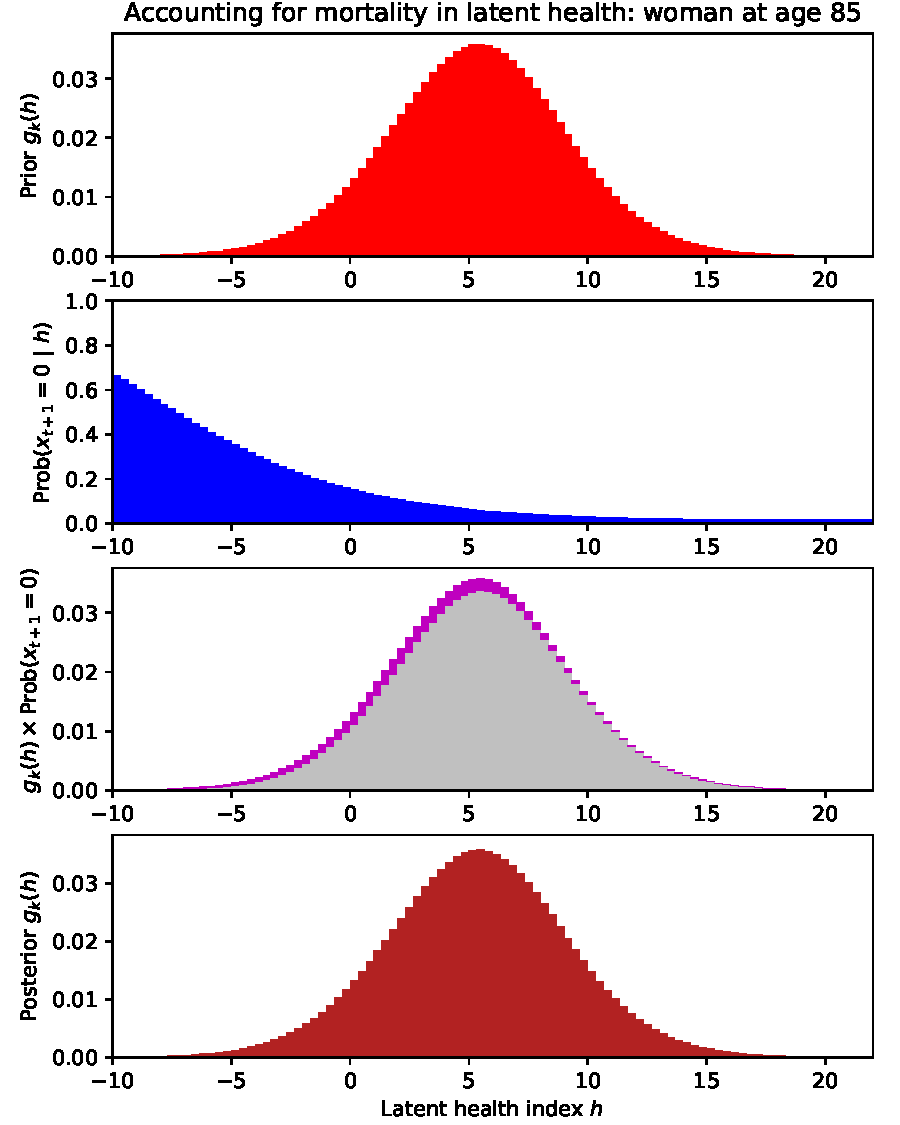
\includegraphics{\FigsDir/MortalityDemo.pdf}
	\caption{Graphical summary of one period's survivorship into the log-likelihood function. Top panel shows prior distribution of latent health; second panel shows mortality probability for each discrete latent health level. Purple area in third panel represents mass of decedents; total size of gray area is survivorship. Bottom panel normalizes gray distribution to generate posterior distribution after accounting for mortality this period.}\label{fig:MortalityDemo}
\end{figure}

From these initial conditions, I iterate over time $t$. If $i$ is observed alive at time $t$, then $\CumLivPrb_i$ is incorporated into $\LL_i$ and reset to one; if $i$ is reported as dead ($\Report_{it} = 0$), the additive complement of $\CumLivPrb_{i}$ is accumulated into $\LL_i$ and its computation is complete.
\begin{equation}\label{LivPrbLL}
\LL_i := \begin{cases}
\LL_{i} + \log(\CumLivPrb_i) & \text{if } \Report_{it} \geq 1 \\
\LL_{i} + \log(1 - \CumLivPrb_i) & \text{if } \Report_{it} = 0 \\
\end{cases}, \qquad \CumLivPrb_i := 1.
\end{equation}
Next, the probability of $i$ reporting $\Report_{it}$ (given the econometrician's distribution $\HealthDstnPcvd_{i}$) is accumulated into $\LL_i$, and the econometrician's distribution is updated using Bayes' rule:
\begin{equation}\label{ReportPrbLL}
\LL_i := \LL_i + \log(\HealthDstnPcvd_{i} \cdot \ReportPrb(\Report_{it})), \qquad \HealthDstnPcvd_{i} := (\HealthDstnPcvd_{i} \odot \ReportPrb(\Report_{it})) / (\HealthDstnPcvd_{i} \cdot \ReportPrb(\Report_{it})).
\end{equation}
If $\Report_{it}$ is not observed this period (e.g.\ because $i$ was not surveyed or refused to answer), then both \eqref{LivPrbLL} and \eqref{ReportPrbLL} are skipped.

To move individual $i$ to period $t+1$, I incorporate the survival probability into $\CumLivPrb_{i}$, then update the  distribution $\HealthDstnPcvd_{i}$ using survival probabilities $\LivPrb_\Age(\Sex_i)$ and the Markov matrix $\overline{\TransPrb}_\Age(\Sex_i)$:
\begin{equation}\label{NextPrdLL}
\CumLivPrb_i := \CumLivPrb_i (\HealthDstnPcvd_{i} \cdot \LivPrb_\Age(\Sex_i)), \qquad \HealthDstnPcvd_{i} := \left[ (\HealthDstnPcvd_{i} \odot \LivPrb_\Age(\Sex_i)) / (\HealthDstnPcvd_{i} \cdot \LivPrb_\Age(\Sex_i)) \right] \times \overline{\TransPrb}_\Age(\Sex_i)^T, \qquad \Age_i := \Age_i + \AgeIncr.
\end{equation}
The incorporation of survivorship into the log-likelihood function is graphically summarized in Figure~\ref{fig:MortalityDemo}, analogous to Figure~\ref{fig:ReportDemo} in the main paper.

The steps in \eqref{LivPrbLL}, \eqref{ReportPrbLL}, and \eqref{NextPrdLL} are repeated until the last observation of $i$ is included in $\LL_i$, incorporating all $Z_i$ reports of categorical health (potentially including an observed death). As usual, the overall log likelihood of the parameter vector $\ParamVec$ given data $\Data$ is the sum across each individual's log likelihood contribution:
\begin{equation}
\mathcal{L}(\ParamVec~|~\Data) = \sum_{i=1}^{I} \LL_i.
\end{equation}


\section{Additional Specifications}\label{app:MoreSpecs}

In the main paper text, I estimate the latent health model on a dataset that combines the Health and Retirement Study (HRS) and the Panel Study of Income Dynamics. The model can alternatively be estimated on each dataset separately, with substantially similar results in terms of model fit and the values of the key parameters. Parameter estimates for the HRS and PSID independently are presented on Tables~\ref{tab:HRSonlyTable} and Tables~\ref{tab:PSIDonlyTable}; some polynomial functions use fewer terms in these specifications.

\begin{table}
\tiny
\singlespace
\begin{center}
\caption{Paramaters Estimated by Maximum Likelihood on HRS Data}\label{tab:HRSonlyTable}
\newsavebox{\HRSonlyTableBox}
\sbox{\HRSonlyTableBox}{  
\begin{tabular}{clccc}
\hline \hline
\rule{0pt}{2.5ex}Param & \multicolumn{1}{c}{Description} & Women & Men & All \\
\hline
\rule{0pt}{2.2ex}$\theta_{0}'$ & Mortality probit: level at model start $\underline{j}$ & 2.467 & 2.105 & 2.405 \\
\rule{0pt}{2.2ex} & & (5.97e-2) & (7.75e-2) & (4.78e-2) \\
\rule{0pt}{2.2ex}$\theta_{s}$ & Mortality probit: shifter for men & 0.00 & 0.00 & -0.222 \\
\rule{0pt}{2.2ex} & & (---) & (---) & (1.34e-2) \\
\rule{0pt}{2.2ex}$\theta_{h1}'$ & Mortality probit: first derivative w.r.t health at $\Health=0$ & 0.125 & 0.191 & 0.156 \\
\rule{0pt}{2.2ex} & & (7.00e-3) & (2.14e-2) & (1.07e-2) \\
\rule{0pt}{2.2ex}$\theta_{h2}'$ & Mortality probit: second derivative w.r.t health at $\Health=0$ & -6.40e-3 & -1.46e-3 & -7.36e-3 \\
\rule{0pt}{2.2ex} & & (1.32e-3) & (3.76e-3) & (1.07e-3) \\
\rule{0pt}{2.2ex}$\theta_{j1}'$ & Mortality probit: first derivative w.r.t age at $\underline{j}$ & -5.78e-2 & -4.75e-2 & -5.18e-2 \\
\rule{0pt}{2.2ex} & & (7.95e-3) & (1.17e-2) & (6.26e-3) \\
\rule{0pt}{2.2ex}$\theta_{j2}'$ & Mortality probit: second derivative w.r.t age at $\underline{j}$ & 2.70e-3 & 2.15e-3 & 2.30e-3 \\
\rule{0pt}{2.2ex} & & (6.57e-4) & (1.03e-3) & (5.18e-4) \\
\rule{0pt}{2.2ex}$\theta_{j3}'$ & Mortality probit: third derivative w.r.t age at $\underline{j}$ & -1.48e-4 & -1.32e-4 & -1.35e-4 \\
\rule{0pt}{2.2ex} & & (2.50e-5) & (4.06e-5) & (1.99e-5) \\
\rule{0pt}{2.2ex}$\theta_{hj}$ & Mortality probit: coefficient on age$\times$health & -3.03e-5 & -7.14e-4 & -3.16e-4 \\
\rule{0pt}{2.2ex} & & (2.13e-5) & (2.50e-4) & (1.18e-4) \\
\rule{0pt}{2.2ex}$\theta_{js}$ & Mortality probit: coefficient on age, adjustment for men & 0.00 & 0.00 & 2.63e-4 \\
\rule{0pt}{2.2ex} & & (---) & (---) & (6.58e-5) \\
\hline
\rule{0pt}{2.2ex}$\gamma_{0}'$ & Correlation factor: level at model start $\underline{j}$ & 3.669 & 3.346 & 3.541 \\
\rule{0pt}{2.2ex} & & (6.78e-2) & (0.102) & (5.93e-2) \\
\rule{0pt}{2.2ex}$\gamma_{j1}'$ & Correlation factor: first derivative w.r.t age at $\underline{j}$ & 5.42e-3 & 2.96e-2 & 1.48e-2 \\
\rule{0pt}{2.2ex} & & (3.44e-3) & (5.98e-3) & (3.38e-3) \\
\hline
\rule{0pt}{2.2ex}$\beta_{0}'$ & Expected health: level at model start $\underline{j}$ & 1.248 & 2.432 & 1.886 \\
\rule{0pt}{2.2ex} & & (0.804) & (0.660) & (0.474) \\
\rule{0pt}{2.2ex}$\beta_{s}$ & Expected health: shifter for men & 0.00 & 0.00 & -0.428 \\
\rule{0pt}{2.2ex} & & (---) & (---) & (0.179) \\
\rule{0pt}{2.2ex}$\beta_{j1}'$ & Expected health: first derivative w.r.t age at $\underline{j}$ & 0.390 & 1.92e-2 & 0.229 \\
\rule{0pt}{2.2ex} & & (0.144) & (0.126) & (7.59e-2) \\
\rule{0pt}{2.2ex}$\beta_{j2}'$ & Expected health: second derivative w.r.t age at $\underline{j}$ & -7.18e-2 & -3.16e-2 & -5.44e-2 \\
\rule{0pt}{2.2ex} & & (1.56e-2) & (1.08e-2) & (8.51e-3) \\
\rule{0pt}{2.2ex}$\beta_{j3}'$ & Expected health: third derivative w.r.t age at $\underline{j}$ & 3.15e-3 & 0.00 & 1.99e-3 \\
\rule{0pt}{2.2ex} & & (7.10e-4) & (---) & (4.40e-4) \\
\rule{0pt}{2.2ex}$\beta_{js}$ & Expected health: coefficient on age, adjustment for men & 0.00 & 0.00 & -1.82e-2 \\
\rule{0pt}{2.2ex} & & (---) & (---) & (8.92e-3) \\
\hline
\rule{0pt}{2.2ex}$\mu_0$ & Mean of initial latent health at $\underline{j}$ & 7.859 & 7.368 & 7.597 \\
\rule{0pt}{2.2ex} & & (0.184) & (0.247) & (0.133) \\
\rule{0pt}{2.2ex}$\sigma_0$ & Standard deviation of initial latent health at $\underline{j}$ & 4.341 & 3.850 & 4.083 \\
\rule{0pt}{2.2ex} & & (0.119) & (0.152) & (8.95e-2) \\
\rule{0pt}{2.2ex}$q_1$ & Health shocks: probability of small shock & 0.956 & 0.959 & 0.959 \\
\rule{0pt}{2.2ex} & & (7.53e-3) & (6.18e-3) & (4.47e-3) \\
\rule{0pt}{2.2ex}$\mu_1$ & Health shocks: mean for small shock & 9.18e-2 & 9.83e-2 & 9.40e-2 \\
\rule{0pt}{2.2ex} & & (8.07e-3) & (6.44e-3) & (4.91e-3) \\
\rule{0pt}{2.2ex}$\sigma_1$ & Health shocks: stdev for small shock & 0.481 & 0.445 & 0.473 \\
\rule{0pt}{2.2ex} & & (3.38e-2) & (2.96e-2) & (2.11e-2) \\
\rule{0pt}{2.2ex}$q_2$ & Health shocks: probability of large shock & 4.36e-2 & 4.11e-2 & 4.09e-2 \\
\rule{0pt}{2.2ex} & & (7.53e-3) & (6.18e-3) & (4.47e-3) \\
\rule{0pt}{2.2ex}$\mu_1$ & Health shocks: mean for large shock & -2.013 & -2.291 & -2.204 \\
\rule{0pt}{2.2ex} & & (0.239) & (0.280) & (0.180) \\
\rule{0pt}{2.2ex}$\sigma_1$ & Health shocks: stdev for large shock & 3.690 & 3.770 & 3.761 \\
\rule{0pt}{2.2ex} & & (0.221) & (0.184) & (0.139) \\
\hline
\rule{0pt}{2.2ex}$p_1$ & Proportion of reporting type 1 individuals & 0.474 & 0.494 & 0.456 \\
\rule{0pt}{2.2ex} & & (1.76e-2) & (2.99e-2) & (5.94e-3) \\
\rule{0pt}{2.2ex}$\varsigma_1$ & Standard deviation of SRHS shocks for type 1 & 1.059 & 0.505 & 1.105 \\
\rule{0pt}{2.2ex} & & (3.99e-2) & (1.88e-2) & (1.99e-2) \\
\rule{0pt}{2.2ex}$p_2$ & Proportion of reporting type 2 individuals & 0.430 & 0.440 & 0.470 \\
\rule{0pt}{2.2ex} & & (2.72e-2) & (2.26e-2) & (6.85e-3) \\
\rule{0pt}{2.2ex}$\varsigma_2$ & Standard deviation of SRHS shocks for type 2 & 0.485 & 1.127 & 0.499 \\
\rule{0pt}{2.2ex} & & (1.71e-2) & (4.07e-2) & (7.17e-3) \\
\rule{0pt}{2.2ex}$p_3$ & Proportion of reporting type 3 individuals & 9.64e-2 & 6.55e-2 & 7.43e-2 \\
\rule{0pt}{2.2ex} & & (2.26e-2) & (1.57e-2) & (1.24e-2) \\
\rule{0pt}{2.2ex}$\varsigma_3$ & Standard deviation of SRHS shocks for type 3 & 1.951 & 2.193 & 2.099 \\
\rule{0pt}{2.2ex} & & (0.104) & (0.135) & (8.80e-2) \\
\hline
\rule{0pt}{2.2ex}$\alpha_1$ & SRHS: Linear coefficient on latent health & 0.463 & 0.481 & 0.472 \\
\rule{0pt}{2.2ex} & & (1.18e-2) & (1.51e-2) & (9.27e-3) \\
\rule{0pt}{2.2ex}$\chi_2$ & SRHS: Cut b/w reporting ``fair'' and ``good'' & 1.780 & 1.740 & 1.757 \\
\rule{0pt}{2.2ex} & & (2.26e-2) & (2.79e-2) & (1.78e-2) \\
\rule{0pt}{2.2ex}$\chi_3$ & SRHS: Cut b/w reporting ``good'' and ``very good'' & 3.488 & 3.377 & 3.430 \\
\rule{0pt}{2.2ex} & & (3.42e-2) & (4.24e-2) & (2.73e-2) \\
\rule{0pt}{2.2ex}$\chi_4$ & SRHS: Cut b/w reporting ``very good'' and ``excellent'' & 5.511 & 5.213 & 5.362 \\
\rule{0pt}{2.2ex} & & (4.94e-2) & (6.05e-2) & (3.94e-2) \\
\hline
\rule{0pt}{2.2ex}$I$ & Number of unique individuals & 20,108 & 16,094 & 36,202\\
\rule{0pt}{2.2ex}$\lVert X \rVert$ & Number of observations of SRHS (alive \& dead) & 113,336 & 86,377 & 199,713\\
\rule{0pt}{2.2ex}$\mathcal{L}(\widehat{\Delta} | X)$ & Log likelihood at estimated parameters & 129,106.9 & 112,893.6 & 242,062.4\\
\hline\hline
\end{tabular}
 } 
\usebox{\HRSonlyTableBox}  
\end{center}
\end{table}


\begin{table}
\tiny
\singlespace
\begin{center}
\caption{Paramaters Estimated by Maximum Likelihood on PSID Data}\label{tab:PSIDonlyTable}
\newsavebox{\PSIDonlyTableBox}
\sbox{\PSIDonlyTableBox}{  
\begin{tabular}{clccc}
\hline \hline
\rule{0pt}{2.5ex}Param & \multicolumn{1}{c}{Description} & Women & Men & All \\
\hline
\rule{0pt}{2.2ex}$\theta_{0}'$ & Mortality probit: level at model start $\underline{j}$ & 2.132 & 2.165 & 2.286 \\
\rule{0pt}{2.2ex} & & (0.123) & (0.104) & (9.95e-2) \\
\rule{0pt}{2.2ex}$\theta_{s}$ & Mortality probit: shifter for men & 0.00 & 0.00 & -0.263 \\
\rule{0pt}{2.2ex} & & (---) & (---) & (0.119) \\
\rule{0pt}{2.2ex}$\theta_{h1}'$ & Mortality probit: first derivative w.r.t health at $\Health=0$ & 0.174 & 0.103 & 0.137 \\
\rule{0pt}{2.2ex} & & (2.28e-2) & (1.47e-2) & (1.65e-2) \\
\rule{0pt}{2.2ex}$\theta_{h2}'$ & Mortality probit: second derivative w.r.t health at $\Health=0$ & -9.57e-3 & -2.21e-3 & -6.08e-3 \\
\rule{0pt}{2.2ex} & & (1.75e-3) & (1.71e-3) & (1.29e-3) \\
\rule{0pt}{2.2ex}$\theta_{j1}'$ & Mortality probit: first derivative w.r.t age at $\underline{j}$ & 1.56e-2 & 3.37e-3 & 8.28e-3 \\
\rule{0pt}{2.2ex} & & (5.16e-3) & (5.08e-3) & (4.09e-3) \\
\rule{0pt}{2.2ex}$\theta_{j2}'$ & Mortality probit: second derivative w.r.t age at $\underline{j}$ & -1.07e-3 & -7.79e-4 & -9.14e-4 \\
\rule{0pt}{2.2ex} & & (1.12e-4) & (1.26e-4) & (8.77e-5) \\
\rule{0pt}{2.2ex}$\theta_{j3}'$ & Mortality probit: third derivative w.r.t age at $\underline{j}$ & 0.00 & 0.00 & 0.00 \\
\rule{0pt}{2.2ex} & & (---) & (---) & (---) \\
\rule{0pt}{2.2ex}$\theta_{hj}$ & Mortality probit: coefficient on age$\times$health & -5.84e-4 & -7.71e-5 & -2.91e-4 \\
\rule{0pt}{2.2ex} & & (2.63e-4) & (1.70e-4) & (2.04e-4) \\
\rule{0pt}{2.2ex}$\theta_{js}$ & Mortality probit: coefficient on age, adjustment for men & 0.00 & 0.00 & 1.13e-3 \\
\rule{0pt}{2.2ex} & & (---) & (---) & (1.75e-3) \\
\hline
\rule{0pt}{2.2ex}$\gamma_{0}'$ & Correlation factor: level at model start $\underline{j}$ & 3.469 & 2.836 & 3.189 \\
\rule{0pt}{2.2ex} & & (0.102) & (0.103) & (0.103) \\
\rule{0pt}{2.2ex}$\gamma_{j1}'$ & Correlation factor: first derivative w.r.t age at $\underline{j}$ & 2.49e-2 & 9.36e-2 & 4.86e-2 \\
\rule{0pt}{2.2ex} & & (4.12e-3) & (8.07e-3) & (9.09e-3) \\
\rule{0pt}{2.2ex}$\gamma_{j2}'$ & Correlation factor: second derivative w.r.t age at $\underline{j}$ & 0.00 & -2.31e-3 & -6.65e-4 \\
\rule{0pt}{2.2ex} & & (---) & (2.50e-4) & (3.01e-4) \\
\hline
\rule{0pt}{2.2ex}$\beta_{0}'$ & Expected health: level at model start $\underline{j}$ & 11.142 & 12.438 & 11.128 \\
\rule{0pt}{2.2ex} & & (0.920) & (0.821) & (0.670) \\
\rule{0pt}{2.2ex}$\beta_{s}$ & Expected health: shifter for men & 0.00 & 0.00 & 2.407 \\
\rule{0pt}{2.2ex} & & (---) & (---) & (0.370) \\
\rule{0pt}{2.2ex}$\beta_{j1}'$ & Expected health: first derivative w.r.t age at $\underline{j}$ & -0.885 & -0.688 & -0.869 \\
\rule{0pt}{2.2ex} & & (0.164) & (0.123) & (0.142) \\
\rule{0pt}{2.2ex}$\beta_{j2}'$ & Expected health: second derivative w.r.t age at $\underline{j}$ & 6.73e-2 & 5.80e-3 & 5.99e-2 \\
\rule{0pt}{2.2ex} & & (1.45e-2) & (4.85e-3) & (1.61e-2) \\
\rule{0pt}{2.2ex}$\beta_{j3}'$ & Expected health: third derivative w.r.t age at $\underline{j}$ & -3.19e-3 & 0.00 & -2.82e-3 \\
\rule{0pt}{2.2ex} & & (6.29e-4) & (---) & (7.81e-4) \\
\rule{0pt}{2.2ex}$\beta_{js}$ & Expected health: coefficient on age, adjustment for men & 0.00 & 0.00 & -0.115 \\
\rule{0pt}{2.2ex} & & (---) & (---) & (2.47e-2) \\
\hline
\rule{0pt}{2.2ex}$\mu_0$ & Mean of initial latent health at $\underline{j}$ & 10.801 & 11.817 & 11.193 \\
\rule{0pt}{2.2ex} & & (0.305) & (0.344) & (0.229) \\
\rule{0pt}{2.2ex}$\sigma_0$ & Standard deviation of initial latent health at $\underline{j}$ & 3.555 & 3.791 & 3.639 \\
\rule{0pt}{2.2ex} & & (0.124) & (0.157) & (0.104) \\
\rule{0pt}{2.2ex}$q_1$ & Health shocks: probability of small shock & 0.941 & 0.928 & 0.934 \\
\rule{0pt}{2.2ex} & & (1.66e-2) & (2.66e-2) & (1.49e-2) \\
\rule{0pt}{2.2ex}$\mu_1$ & Health shocks: mean for small shock & 6.99e-2 & 0.102 & 8.49e-2 \\
\rule{0pt}{2.2ex} & & (1.28e-2) & (1.92e-2) & (1.11e-2) \\
\rule{0pt}{2.2ex}$\sigma_1$ & Health shocks: stdev for small shock & 0.457 & 0.354 & 0.415 \\
\rule{0pt}{2.2ex} & & (8.31e-2) & (0.164) & (7.98e-2) \\
\rule{0pt}{2.2ex}$q_2$ & Health shocks: probability of large shock & 5.93e-2 & 7.24e-2 & 6.58e-2 \\
\rule{0pt}{2.2ex} & & (1.66e-2) & (2.66e-2) & (1.49e-2) \\
\rule{0pt}{2.2ex}$\mu_1$ & Health shocks: mean for large shock & -1.109 & -1.302 & -1.204 \\
\rule{0pt}{2.2ex} & & (0.214) & (0.321) & (0.183) \\
\rule{0pt}{2.2ex}$\sigma_1$ & Health shocks: stdev for large shock & 3.499 & 3.223 & 3.346 \\
\rule{0pt}{2.2ex} & & (0.323) & (0.351) & (0.237) \\
\hline
\rule{0pt}{2.2ex}$p_1$ & Proportion of reporting type 1 individuals & 9.82e-2 & 0.464 & 9.67e-2 \\
\rule{0pt}{2.2ex} & & (2.56e-2) & (2.70e-2) & (1.59e-2) \\
\rule{0pt}{2.2ex}$\varsigma_1$ & Standard deviation of SRHS shocks for type 1 & 1.956 & 1.018 & 2.008 \\
\rule{0pt}{2.2ex} & & (0.120) & (3.53e-2) & (8.26e-2) \\
\rule{0pt}{2.2ex}$p_2$ & Proportion of reporting type 2 individuals & 0.459 & 0.438 & 0.453 \\
\rule{0pt}{2.2ex} & & (3.88e-2) & (3.05e-2) & (3.21e-2) \\
\rule{0pt}{2.2ex}$\varsigma_2$ & Standard deviation of SRHS shocks for type 2 & 0.496 & 0.494 & 0.496 \\
\rule{0pt}{2.2ex} & & (2.35e-2) & (2.10e-2) & (1.88e-2) \\
\rule{0pt}{2.2ex}$p_3$ & Proportion of reporting type 3 individuals & 0.443 & 9.80e-2 & 0.451 \\
\rule{0pt}{2.2ex} & & (3.08e-2) & (1.67e-2) & (2.54e-2) \\
\rule{0pt}{2.2ex}$\varsigma_3$ & Standard deviation of SRHS shocks for type 3 & 1.074 & 2.050 & 1.052 \\
\rule{0pt}{2.2ex} & & (5.07e-2) & (9.63e-2) & (3.69e-2) \\
\hline
\rule{0pt}{2.2ex}$\alpha_1$ & SRHS: Linear coefficient on latent health & 0.413 & 0.389 & 0.403 \\
\rule{0pt}{2.2ex} & & (1.35e-2) & (1.37e-2) & (9.66e-3) \\
\rule{0pt}{2.2ex}$\chi_2$ & SRHS: Cut b/w reporting ``fair'' and ``good'' & 1.714 & 1.728 & 1.722 \\
\rule{0pt}{2.2ex} & & (3.56e-2) & (4.21e-2) & (2.73e-2) \\
\rule{0pt}{2.2ex}$\chi_3$ & SRHS: Cut b/w reporting ``good'' and ``very good'' & 3.595 & 3.516 & 3.561 \\
\rule{0pt}{2.2ex} & & (5.40e-2) & (6.38e-2) & (4.14e-2) \\
\rule{0pt}{2.2ex}$\chi_4$ & SRHS: Cut b/w reporting ``very good'' and ``excellent'' & 5.445 & 5.213 & 5.336 \\
\rule{0pt}{2.2ex} & & (7.20e-2) & (8.26e-2) & (5.44e-2) \\
\hline
\rule{0pt}{2.2ex}$I$ & Number of unique individuals & 11,787 & 10,791 & 22,578\\
\rule{0pt}{2.2ex}$\lVert X \rVert$ & Number of observations of SRHS (alive \& dead) & 70,341 & 59,311 & 129,652\\
\rule{0pt}{2.2ex}$\mathcal{L}(\widehat{\Delta} | X)$ & Log likelihood at estimated parameters & 86,745.2 & 74,575.4 & 160,129.6\\
\hline\hline
\end{tabular}
 } 
\usebox{\PSIDonlyTableBox} 
\end{center}
\end{table}


\begin{table}
\tiny
\singlespace
\begin{center}
\caption{Paramaters Estimated by Maximum Likelihood on MEPS Data}\label{tab:MEPSonlyTable}
\newsavebox{\MEPSonlyTableBox}
\sbox{\MEPSonlyTableBox}{  
\begin{tabular}{clccc}
\hline \hline
\rule{0pt}{2.5ex}Param & \multicolumn{1}{c}{Description} & Women & Men & All \\
\hline
\rule{0pt}{2.2ex}$\theta_{0}'$ & Mortality probit: level at model start $\underline{j}$ & 2.676 & 2.429 & 2.658 \\
\rule{0pt}{2.2ex} & & (9.52e-2) & (6.75e-2) & (0.169) \\
\rule{0pt}{2.2ex}$\theta_{s}$ & Mortality probit: shifter for men & 0.00 & 0.00 & -0.272 \\
\rule{0pt}{2.2ex} & & (---) & (---) & (0.113) \\
\rule{0pt}{2.2ex}$\theta_{h1}'$ & Mortality probit: first derivative w.r.t health at $\Health=0$ & 0.139 & 9.81e-2 & 0.119 \\
\rule{0pt}{2.2ex} & & (1.11e-2) & (9.50e-3) & (4.64e-3) \\
\rule{0pt}{2.2ex}$\theta_{h2}'$ & Mortality probit: second derivative w.r.t health at $\Health=0$ & 4.80e-3 & 1.10e-2 & 7.72e-3 \\
\rule{0pt}{2.2ex} & & (1.56e-3) & (2.89e-3) & (2.69e-3) \\
\rule{0pt}{2.2ex}$\theta_{j1}'$ & Mortality probit: first derivative w.r.t age at $\underline{j}$ & 6.01e-3 & 1.45e-2 & 1.01e-2 \\
\rule{0pt}{2.2ex} & & (3.59e-3) & (4.03e-3) & (1.26e-2) \\
\rule{0pt}{2.2ex}$\theta_{j2}'$ & Mortality probit: second derivative w.r.t age at $\underline{j}$ & -8.05e-4 & -1.34e-3 & -1.07e-3 \\
\rule{0pt}{2.2ex} & & (9.02e-5) & (2.45e-4) & (6.32e-4) \\
\rule{0pt}{2.2ex}$\theta_{j3}'$ & Mortality probit: third derivative w.r.t age at $\underline{j}$ & 3.18e-6 & 1.71e-5 & 9.43e-6 \\
\rule{0pt}{2.2ex} & & (3.72e-6) & (7.25e-6) & (1.53e-5) \\
\rule{0pt}{2.2ex}$\theta_{hj}$ & Mortality probit: coefficient on age$\times$health & -1.40e-4 & 3.33e-4 & 1.04e-4 \\
\rule{0pt}{2.2ex} & & (1.45e-4) & (1.10e-4) & (1.50e-5) \\
\rule{0pt}{2.2ex}$\theta_{js}$ & Mortality probit: coefficient on age, adjustment for men & 0.00 & 0.00 & 1.45e-3 \\
\rule{0pt}{2.2ex} & & (---) & (---) & (1.78e-3) \\
\hline
\rule{0pt}{2.2ex}$\gamma_{0}'$ & Correlation factor: level at model start $\underline{j}$ & 2.509 & 2.507 & 2.480 \\
\rule{0pt}{2.2ex} & & (3.99e-2) & (3.61e-2) & (2.36e-2) \\
\rule{0pt}{2.2ex}$\gamma_{j1}'$ & Correlation factor: first derivative w.r.t age at $\underline{j}$ & 4.10e-2 & 1.72e-2 & 3.17e-2 \\
\rule{0pt}{2.2ex} & & (4.99e-3) & (2.73e-3) & (1.38e-3) \\
\rule{0pt}{2.2ex}$\gamma_{j2}'$ & Correlation factor: second derivative w.r.t age at $\underline{j}$ & -1.23e-3 & 6.12e-4 & -4.79e-4 \\
\rule{0pt}{2.2ex} & & (3.80e-4) & (1.92e-4) & (4.82e-5) \\
\rule{0pt}{2.2ex}$\gamma_{j3}'$ & Correlation factor: third derivative w.r.t age at $\underline{j}$ & 1.67e-5 & -3.48e-5 & -4.74e-6 \\
\rule{0pt}{2.2ex} & & (1.23e-5) & (6.73e-6) & (9.72e-7) \\
\hline
\rule{0pt}{2.2ex}$\beta_{0}'$ & Expected health: level at model start $\underline{j}$ & 7.972 & 8.102 & 7.638 \\
\rule{0pt}{2.2ex} & & (0.147) & (0.140) & (9.41e-2) \\
\rule{0pt}{2.2ex}$\beta_{s}$ & Expected health: shifter for men & 0.00 & 0.00 & 0.713 \\
\rule{0pt}{2.2ex} & & (---) & (---) & (3.80e-2) \\
\rule{0pt}{2.2ex}$\beta_{j1}'$ & Expected health: first derivative w.r.t age at $\underline{j}$ & 0.127 & 0.126 & 0.134 \\
\rule{0pt}{2.2ex} & & (3.22e-2) & (2.68e-2) & (1.78e-2) \\
\rule{0pt}{2.2ex}$\beta_{j2}'$ & Expected health: second derivative w.r.t age at $\underline{j}$ & -2.54e-2 & -2.57e-2 & -2.52e-2 \\
\rule{0pt}{2.2ex} & & (4.41e-3) & (3.71e-3) & (2.45e-3) \\
\rule{0pt}{2.2ex}$\beta_{j3}'$ & Expected health: third derivative w.r.t age at $\underline{j}$ & 1.92e-3 & 1.91e-3 & 1.90e-3 \\
\rule{0pt}{2.2ex} & & (3.33e-4) & (2.86e-4) & (1.87e-4) \\
\rule{0pt}{2.2ex}$\beta_{j3}'$ & Expected health: fourth derivative w.r.t age at $\underline{j}$ & -6.47e-5 & -6.46e-5 & -6.41e-5 \\
\rule{0pt}{2.2ex} & & (1.11e-5) & (9.79e-6) & (6.27e-6) \\
\rule{0pt}{2.2ex}$\beta_{js}$ & Expected health: coefficient on age, adjustment for men & 0.00 & 0.00 & -2.15e-2 \\
\rule{0pt}{2.2ex} & & (---) & (---) & (1.64e-3) \\
\hline
\rule{0pt}{2.2ex}$\mu_0$ & Mean of initial latent health at $\underline{j}$ & 9.786 & 10.027 & 9.850 \\
\rule{0pt}{2.2ex} & & (0.116) & (0.139) & (9.41e-2) \\
\rule{0pt}{2.2ex}$\sigma_0$ & Standard deviation of initial latent health at $\underline{j}$ & 2.963 & 2.661 & 2.819 \\
\rule{0pt}{2.2ex} & & (5.73e-2) & (5.33e-2) & (3.97e-2) \\
\rule{0pt}{2.2ex}$q_1$ & Health shocks: probability of small shock & 0.932 & 0.939 & 0.935 \\
\rule{0pt}{2.2ex} & & (5.75e-3) & (4.96e-3) & (3.64e-3) \\
\rule{0pt}{2.2ex}$\mu_1$ & Health shocks: mean for small shock & 6.08e-2 & 5.09e-2 & 5.64e-2 \\
\rule{0pt}{2.2ex} & & (3.01e-3) & (3.22e-3) & (2.27e-3) \\
\rule{0pt}{2.2ex}$\sigma_1$ & Health shocks: stdev for small shock & 0.414 & 0.479 & 0.453 \\
\rule{0pt}{2.2ex} & & (3.01e-2) & (2.41e-2) & (1.82e-2) \\
\rule{0pt}{2.2ex}$q_2$ & Health shocks: probability of large shock & 6.76e-2 & 6.11e-2 & 6.54e-2 \\
\rule{0pt}{2.2ex} & & (5.75e-3) & (4.96e-3) & (3.64e-3) \\
\rule{0pt}{2.2ex}$\mu_1$ & Health shocks: mean for large shock & -0.838 & -0.783 & -0.805 \\
\rule{0pt}{2.2ex} & & (6.75e-2) & (7.64e-2) & (5.01e-2) \\
\rule{0pt}{2.2ex}$\sigma_1$ & Health shocks: stdev for large shock & 3.418 & 3.491 & 3.415 \\
\rule{0pt}{2.2ex} & & (9.69e-2) & (9.55e-2) & (6.37e-2) \\
\hline
\rule{0pt}{2.2ex}$p_1$ & Proportion of reporting type 1 individuals & 6.19e-2 & 5.96e-2 & 6.12e-2 \\
\rule{0pt}{2.2ex} & & (5.13e-2) & (1.44e-2) & (1.35e-2) \\
\rule{0pt}{2.2ex}$\varsigma_1$ & Standard deviation of SRHS shocks for type 1 & 1.950 & 1.975 & 1.960 \\
\rule{0pt}{2.2ex} & & (0.288) & (9.30e-2) & (8.05e-2) \\
\rule{0pt}{2.2ex}$p_2$ & Proportion of reporting type 2 individuals & 0.452 & 0.435 & 0.444 \\
\rule{0pt}{2.2ex} & & (2.75e-2) & (1.16e-2) & (9.36e-3) \\
\rule{0pt}{2.2ex}$\varsigma_2$ & Standard deviation of SRHS shocks for type 2 & 0.466 & 0.452 & 0.459 \\
\rule{0pt}{2.2ex} & & (1.51e-2) & (8.39e-3) & (6.10e-3) \\
\rule{0pt}{2.2ex}$p_3$ & Proportion of reporting type 3 individuals & 0.486 & 0.505 & 0.495 \\
\rule{0pt}{2.2ex} & & (2.66e-2) & (1.14e-2) & (8.80e-3) \\
\rule{0pt}{2.2ex}$\varsigma_3$ & Standard deviation of SRHS shocks for type 3 & 1.171 & 1.159 & 1.165 \\
\rule{0pt}{2.2ex} & & (7.09e-2) & (2.15e-2) & (1.97e-2) \\
\hline
\rule{0pt}{2.2ex}$\alpha_1$ & SRHS: Linear coefficient on latent health & 0.482 & 0.497 & 0.494 \\
\rule{0pt}{2.2ex} & & (5.94e-3) & (7.72e-3) & (5.25e-3) \\
\rule{0pt}{2.2ex}$\chi_2$ & SRHS: Cut b/w reporting ``fair'' and ``good'' & 1.753 & 1.726 & 1.742 \\
\rule{0pt}{2.2ex} & & (1.17e-2) & (1.30e-2) & (8.72e-3) \\
\rule{0pt}{2.2ex}$\chi_3$ & SRHS: Cut b/w reporting ``good'' and ``very good'' & 3.521 & 3.508 & 3.518 \\
\rule{0pt}{2.2ex} & & (1.59e-2) & (1.75e-2) & (1.19e-2) \\
\rule{0pt}{2.2ex}$\chi_4$ & SRHS: Cut b/w reporting ``very good'' and ``excellent'' & 5.060 & 4.963 & 5.016 \\
\rule{0pt}{2.2ex} & & (1.92e-2) & (2.11e-2) & (1.44e-2) \\
\hline
\rule{0pt}{2.2ex}$I$ & Number of unique individuals & 126,486 & 110,044 & 236,530\\
\rule{0pt}{2.2ex}$\lVert X \rVert$ & Number of observations of SRHS (alive \& dead) & 602,881 & 519,891 & 1,122,772\\
\rule{0pt}{2.2ex}$\mathcal{L}(\widehat{\Delta} | X)$ & Log likelihood at estimated parameters & 710,513.6 & 659,142.7 & 1,369,948.4\\
\hline\hline
\end{tabular}
 } 
\usebox{\MEPSonlyTableBox}  
\end{center}
\end{table}


The model can also be estimated on data from the Medical Expenditure Panel Study (MEPS), also yielding comparable results (see Table~\ref{tab:MEPSonlyTable}). The MEPS is a short panel survey focusing on medical events and expenses incurred through them.  Respondents are interviewed every six months over a two year span, for a total of five waves; just under 90\% of individuals in the MEPS are interviewed and report their SRHS in all five waves.  A new MEPS panel begins every year, so two overlapping panels are interviewed in each data wave.  Households heads of any age can be selected for the MEPS, and the SRHS question is asked for all members of a sample household.  The dataset constructed for this paper uses Panels 1 through 20, spanning 1996 to 2016.

The SRHS question for the MEPS reads: ``In general, compared to other people of your age, would you say that your health is excellent, very good, good, fair, or poor?''  Of the three surveys used for this paper, the MEPS is the only one to qualify SRHS with a reference to the individual's age, possibly yielding different results and reducing comparability with the PSID and HRS.  In addition to the standard five waves, the MEPS also mails a short self-administered questionnaire (SAQ) to all respondents a few weeks after their second and fourth wave interviews. The MEPS-SAQ includes a SRHS question that is worded nearly identically to that of the PSID and HRS.

Although the latent health model can be applied to minors, the motivation of the paper is to provide a more accurate health process for dynamic structural models, which usually have agents that begin no earlier than age 18.  I thus set the age of model entry (denoted $\AgeMin$ in Section \ref{sec:Model}) at 18, ignoring any observations at younger ages.\footnote{MEPS respondents thus might ``age into'' the sample in the middle of their panel.}  The MEPS censors respondents age at 85, so I drop all individuals who report this in their first wave, as their true age cannot be known.  To match the structure of the survey, the age increment for the model is $\AgeIncr=0.5$ years.  Each respondent's age in their first observed wave is incremented by half a year if they report being older in the second wave six months later.

Even with its short duration, the MEPS dataset is by far the largest constructed for this paper, both by number of individuals (about 236,000) and total observed waves (over 1.1 million).  Just under 90\% of MEPS respondents are observed in all five waves of their panel; the majority of the remainder are observed for exactly three periods (one year), possibly representing planned attrition by the survey designers.  However, because the vast majority of respondents are non-elderly and relatively healthy and are observed for only two years, fewer than 2,500 deaths are observed for men and women combined.

In the main paper text, I show that the model's expectation of latent health predicts retirement behavior almost exactly as well as a more general specification with age dummies and a full interaction of SRHS over two waves.  The MEPS includes detailed and accurate medical spending data for its respondents, and thus can be used to test SRHS's ability to predict medical costs. For each MEPS respondent who appears in all five waves, I calculate $\widehat{\Health}_{it}$ and $\widehat{\Health^2}_{it}$ as the expectation of $\Health_{it}$ and $\Health^2_{it}$ respectively given their posterior distribution after observing SRHS in the first three waves.  I then regress log total medical costs between waves 3 and 5 (i.e.\ for the year after the three observations of SRHS) on a cubic of age, $\widehat{\Health}_{it}$ and $\widehat{\Health^2}_{it}$.  For the 98,455 MEPS women with positive medical costs, the $R^2$ of this regression is 0.161, very slightly higher than that reached by regressing log medical spending on a \textit{full set} of dummies for the interaction of age and SRHS in wave 3; for men (sample size of 71,084), the $R^2$ is higher at 0.235, but also slightly better than the performance of the full interaction specification.\footnote{The adjusted $R^2$ for the full interaction specification is even lower, as it includes about 335 dummies.} As with predicting retirement behavior, a parametric model based on expected latent health performs at least as well as a much more flexible model using SRHS alone.

\begin{table}
\tiny
\singlespace
\begin{center}
\caption{Paramaters Estimated by Maximum Likelihood on HRS and PSID Data, Basic Model}\label{tab:BasicTable}
\newsavebox{\BasicTableBox}
\sbox{\BasicTableBox}{  
\begin{tabular}{clccc}
\hline \hline
\rule{0pt}{2.5ex}Param & \multicolumn{1}{c}{Description} & Women & Men & All \\
\hline
\rule{0pt}{2.2ex}$\theta_{0}'$ & Mortality probit: level at model start $\underline{j}$ & 2.798 & 2.363 & 2.701 \\
\rule{0pt}{2.2ex} & & (0.151) & (6.85e-2) & (7.58e-2) \\
\rule{0pt}{2.2ex}$\theta_{s}$ & Mortality probit: shifter for men & 0.00 & 0.00 & -0.275 \\
\rule{0pt}{2.2ex} & & (---) & (---) & (6.10e-2) \\
\rule{0pt}{2.2ex}$\theta_{h1}'$ & Mortality probit: first derivative w.r.t health at $\Health=0$ & 0.103 & 0.116 & 0.109 \\
\rule{0pt}{2.2ex} & & (7.14e-3) & (5.90e-3) & (3.92e-3) \\
\rule{0pt}{2.2ex}$\theta_{h2}'$ & Mortality probit: second derivative w.r.t health at $\Health=0$ & -4.09e-3 & -4.11e-3 & -4.01e-3 \\
\rule{0pt}{2.2ex} & & (1.01e-3) & (1.11e-3) & (7.40e-4) \\
\rule{0pt}{2.2ex}$\theta_{j1}'$ & Mortality probit: first derivative w.r.t age at $\underline{j}$ & -2.44e-2 & -1.12e-2 & -1.80e-2 \\
\rule{0pt}{2.2ex} & & (1.04e-2) & (2.17e-3) & (4.98e-3) \\
\rule{0pt}{2.2ex}$\theta_{j2}'$ & Mortality probit: second derivative w.r.t age at $\underline{j}$ & 5.41e-4 & -3.79e-5 & 2.48e-4 \\
\rule{0pt}{2.2ex} & & (4.75e-4) & (1.52e-5) & (2.40e-4) \\
\rule{0pt}{2.2ex}$\theta_{j3}'$ & Mortality probit: third derivative w.r.t age at $\underline{j}$ & -3.34e-5 & -2.00e-5 & -2.68e-5 \\
\rule{0pt}{2.2ex} & & (1.06e-5) & (1.97e-6) & (5.65e-6) \\
\rule{0pt}{2.2ex}$\theta_{hj}$ & Mortality probit: coefficient on age$\times$health & 8.63e-5 & 5.02e-6 & 3.66e-5 \\
\rule{0pt}{2.2ex} & & (6.68e-5) & (4.38e-7) & (1.20e-5) \\
\rule{0pt}{2.2ex}$\theta_{js}$ & Mortality probit: coefficient on age, adjustment for men & 0.00 & 0.00 & 1.02e-3 \\
\rule{0pt}{2.2ex} & & (---) & (---) & (8.20e-4) \\
\hline
\rule{0pt}{2.2ex}$\gamma_{0}'$ & Correlation factor: level at model start $\underline{j}$ & 3.023 & 3.149 & 3.027 \\
\rule{0pt}{2.2ex} & & (0.131) & (0.156) & (9.83e-2) \\
\rule{0pt}{2.2ex}$\gamma_{j1}'$ & Correlation factor: first derivative w.r.t age at $\underline{j}$ & 0.102 & 6.68e-2 & 9.12e-2 \\
\rule{0pt}{2.2ex} & & (1.34e-2) & (1.56e-2) & (1.02e-2) \\
\rule{0pt}{2.2ex}$\gamma_{j2}'$ & Correlation factor: second derivative w.r.t age at $\underline{j}$ & -6.43e-3 & -4.08e-3 & -5.67e-3 \\
\rule{0pt}{2.2ex} & & (8.39e-4) & (9.41e-4) & (6.36e-4) \\
\rule{0pt}{2.2ex}$\gamma_{j3}'$ & Correlation factor: third derivative w.r.t age at $\underline{j}$ & 1.67e-4 & 1.09e-4 & 1.49e-4 \\
\rule{0pt}{2.2ex} & & (2.40e-5) & (2.59e-5) & (1.79e-5) \\
\hline
\rule{0pt}{2.2ex}$\beta_{0}'$ & Expected health: level at model start $\underline{j}$ & 10.777 & 12.100 & 11.173 \\
\rule{0pt}{2.2ex} & & (0.653) & (0.821) & (0.498) \\
\rule{0pt}{2.2ex}$\beta_{s}$ & Expected health: shifter for men & 0.00 & 0.00 & 0.874 \\
\rule{0pt}{2.2ex} & & (---) & (---) & (0.183) \\
\rule{0pt}{2.2ex}$\beta_{j1}'$ & Expected health: first derivative w.r.t age at $\underline{j}$ & -0.734 & -0.919 & -0.827 \\
\rule{0pt}{2.2ex} & & (0.108) & (0.132) & (8.23e-2) \\
\rule{0pt}{2.2ex}$\beta_{j2}'$ & Expected health: second derivative w.r.t age at $\underline{j}$ & 4.51e-2 & 5.81e-2 & 5.29e-2 \\
\rule{0pt}{2.2ex} & & (8.49e-3) & (1.03e-2) & (6.51e-3) \\
\rule{0pt}{2.2ex}$\beta_{j3}'$ & Expected health: third derivative w.r.t age at $\underline{j}$ & -1.46e-3 & -1.94e-3 & -1.73e-3 \\
\rule{0pt}{2.2ex} & & (2.85e-4) & (3.46e-4) & (2.19e-4) \\
\rule{0pt}{2.2ex}$\beta_{js}$ & Expected health: coefficient on age, adjustment for men & 0.00 & 0.00 & -4.54e-2 \\
\rule{0pt}{2.2ex} & & (---) & (---) & (6.67e-3) \\
\hline
\rule{0pt}{2.2ex}$\mu_0$ & Mean of latent health at $\underline{j}$ & 10.449 & 10.734 & 10.581 \\
\rule{0pt}{2.2ex} & & (0.191) & (0.231) & (0.148) \\
\rule{0pt}{2.2ex}$\sigma_{0}$ & Standard deviation of latent health at $\underline{j}$ & 3.752 & 3.648 & 3.747 \\
\rule{0pt}{2.2ex} & & (0.113) & (0.131) & (8.63e-2) \\
\hline
\rule{0pt}{2.2ex}$\alpha_1$ & SRHS: Linear coefficient on latent health & 0.442 & 0.432 & 0.437 \\
\rule{0pt}{2.2ex} & & (7.88e-3) & (9.35e-3) & (6.03e-3) \\
\rule{0pt}{2.2ex}$\chi_2$ & SRHS: Cut b/w reporting ``fair'' and ``good'' & 1.720 & 1.627 & 1.679 \\
\rule{0pt}{2.2ex} & & (1.66e-2) & (1.87e-2) & (1.24e-2) \\
\rule{0pt}{2.2ex}$\chi_3$ & SRHS: Cut b/w reporting ``good'' and ``very good'' & 3.593 & 3.423 & 3.517 \\
\rule{0pt}{2.2ex} & & (2.57e-2) & (2.91e-2) & (1.93e-2) \\
\rule{0pt}{2.2ex}$\chi_4$ & SRHS: Cut b/w reporting ``very good'' and ``excellent'' & 5.720 & 5.389 & 5.567 \\
\rule{0pt}{2.2ex} & & (3.71e-2) & (4.14e-2) & (2.77e-2) \\
\hline
\rule{0pt}{2.2ex}$I$ & Number of unique individuals & 31,803 & 26,832 & 58,635\\
\rule{0pt}{2.2ex}$\lVert X \rVert$ & Number of observations of SRHS (alive \& dead) & 190,623 & 146,919 & 337,542\\
\rule{0pt}{2.2ex}$\mathcal{L}(\widehat{\Delta} | X)$ & Log likelihood at estimated parameters & 229,393.2 & 194,931.8 & 424,485.8\\
\hline\hline
\end{tabular}
 } 
\usebox{\BasicTableBox}  
\end{center}
\end{table}


\begin{figure}
	\centering
	\begin{subfigure}[b]{0.48\textwidth}
		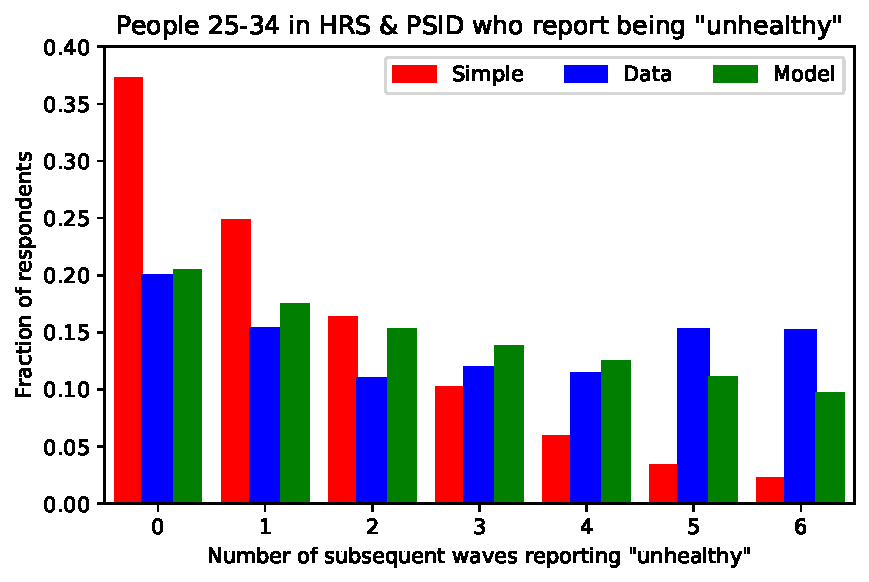
\includegraphics[width=\textwidth]{\FigsDir/TwoStudyOver23basicAllSRHSfreqU25to34.pdf}
		\caption{``Unhealthy'' aged 25-34 at baseline}\label{fig:SRHSfreqU25to34basic}
	\end{subfigure}
	~
	\begin{subfigure}[b]{0.48\textwidth}
		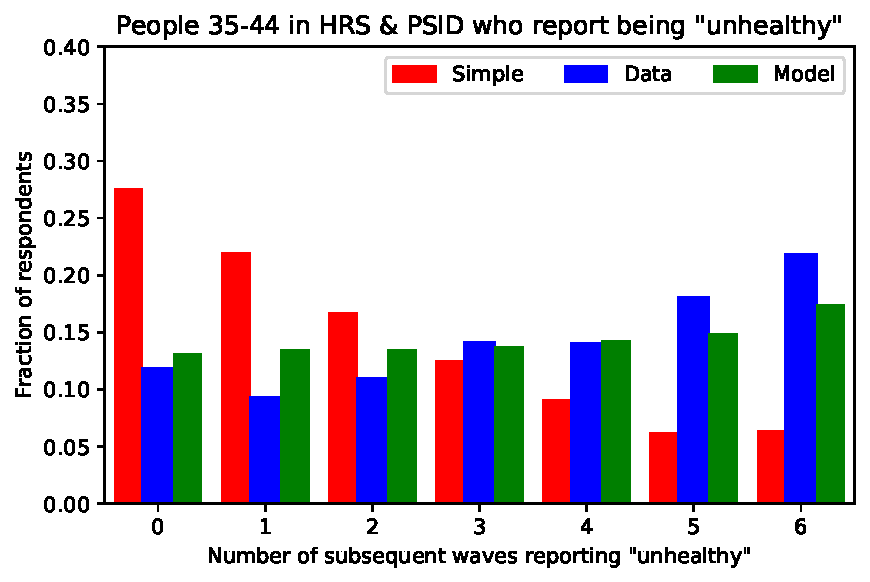
\includegraphics[width=\textwidth]{\FigsDir/TwoStudyOver23basicAllSRHSfreqU35to44.pdf}
		\caption{``Unhealthy'' aged 35-44 at baseline}\label{fig:SRHSfreqU35to44basic}
	\end{subfigure}
	
	\begin{subfigure}[b]{0.48\textwidth}
		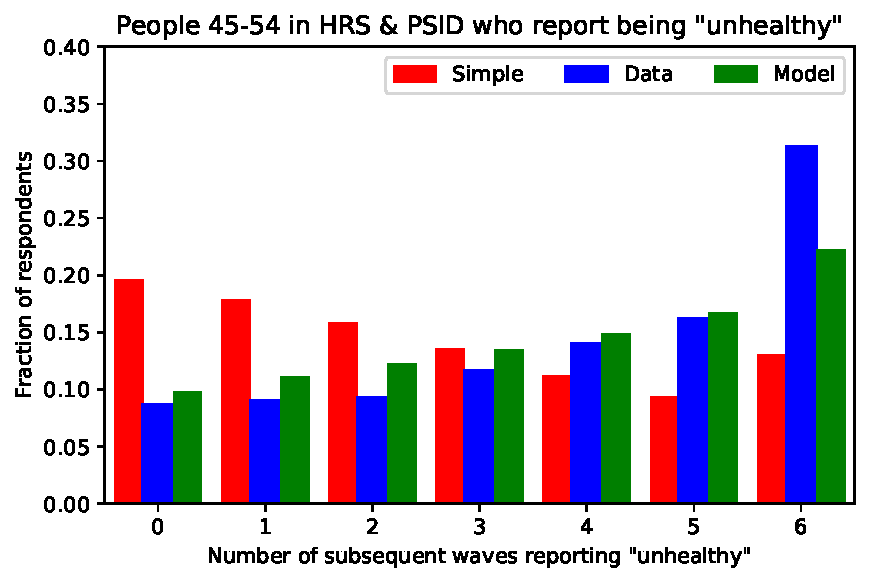
\includegraphics[width=\textwidth]{\FigsDir/TwoStudyOver23basicAllSRHSfreqU45to54.pdf}
		\caption{``Unhealthy'' aged 45-54 at baseline}\label{fig:SRHSfreqU45to54basic}
	\end{subfigure}
	~
	\begin{subfigure}[b]{0.48\textwidth}
		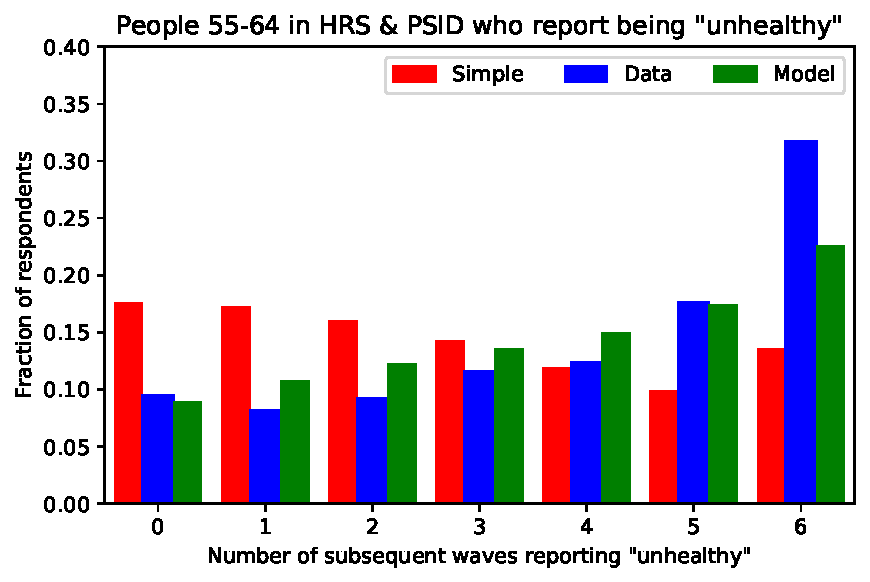
\includegraphics[width=\textwidth]{\FigsDir/TwoStudyOver23basicAllSRHSfreqU55to64.pdf}
		\caption{``Unhealthy'' aged 55-64 at baseline}\label{fig:SRHSfreqU55to64basic}
	\end{subfigure}
	
	
	\begin{subfigure}[b]{0.48\textwidth}
		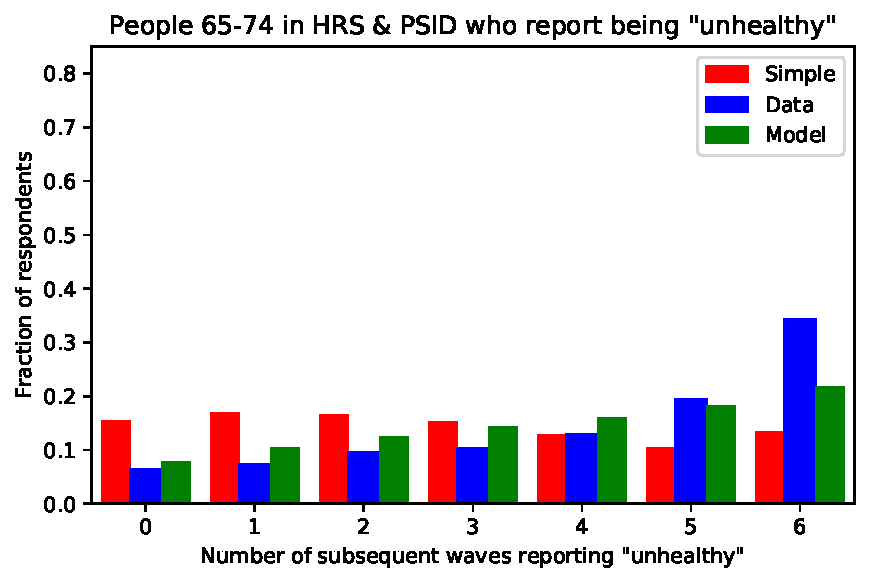
\includegraphics[width=\textwidth]{\FigsDir/TwoStudyOver23basicAllSRHSfreqU65to74.pdf}
		\caption{``Unhealthy'' aged 65-74 at baseline}\label{fig:SRHSfreqU65to74basic}
	\end{subfigure}
	~
	\begin{subfigure}[b]{0.48\textwidth}
		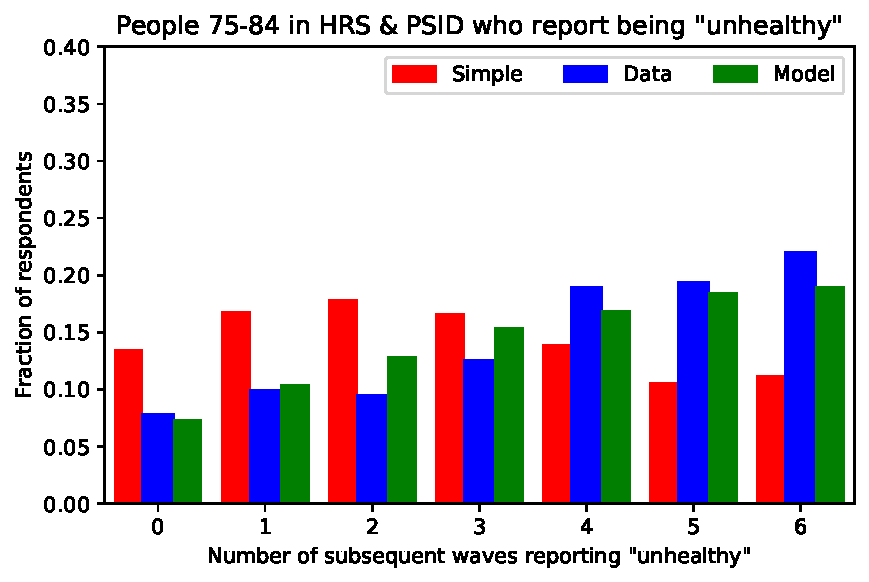
\includegraphics[width=\textwidth]{\FigsDir/TwoStudyOver23basicAllSRHSfreqU75to84.pdf}
		\caption{``Unhealthy'' aged 75-84 at baseline}\label{fig:SRHSfreqU75to84basic}
	\end{subfigure}
	\caption{Distribution of number of times reporting unhealthy SRHS by age and health over next six waves conditional on being unhealthy at baseline, data vs estimated model vs simple dynamics. Basic model version assumes standard normal latent health shocks and no reporting error heterogeneity. Basic model under-predicts the frequency of respondents who are consistently in bad health.}\label{fig:SRHSfreqUTwoStudybasic}
\end{figure}


\begin{figure}
	\centering
	\begin{subfigure}[b]{0.48\textwidth}
		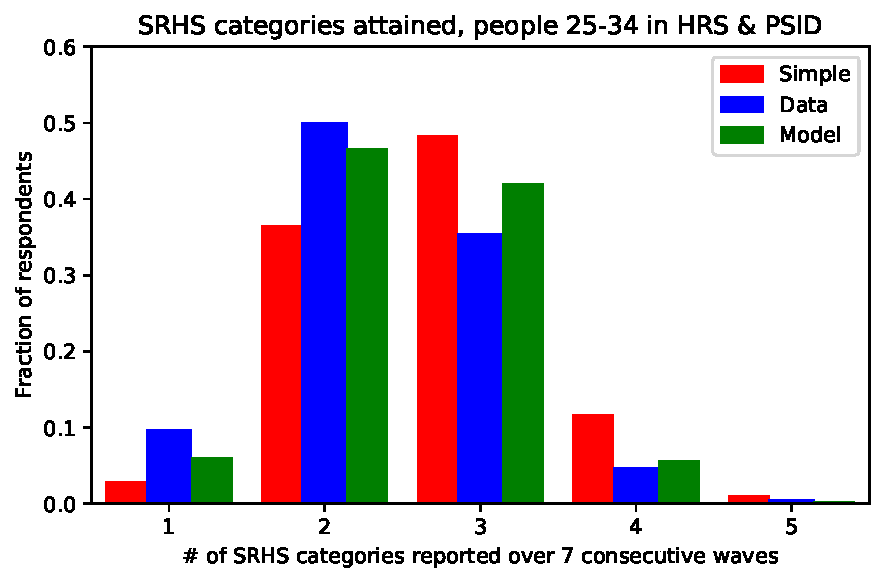
\includegraphics[width=\textwidth]{\FigsDir/TwoStudyOver23basicAllStateCount25to34.pdf}
		\caption{Ages 25-34 at baseline}\label{fig:StateCount25to34basic}
	\end{subfigure}
	~
	\begin{subfigure}[b]{0.48\textwidth}
		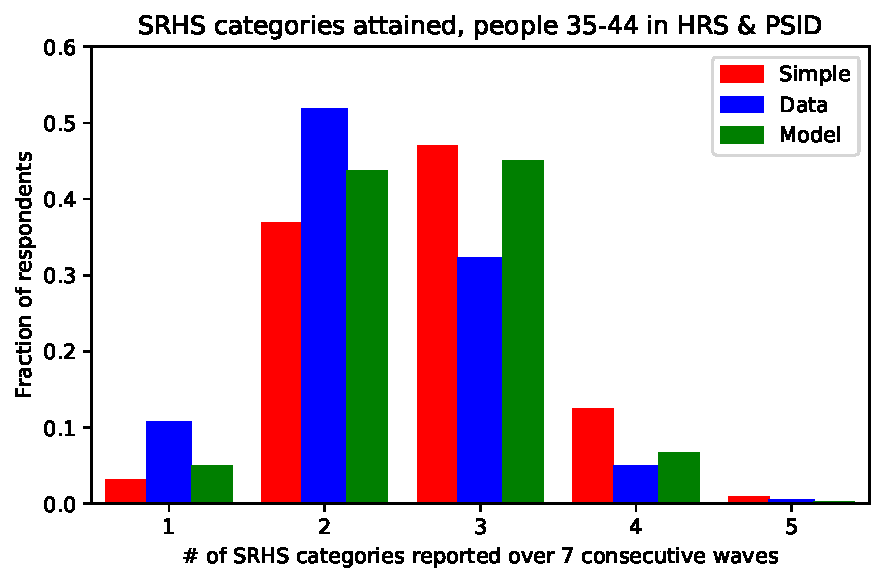
\includegraphics[width=\textwidth]{\FigsDir/TwoStudyOver23basicAllStateCount35to44.pdf}
		\caption{Ages 35-44 at baseline}\label{fig:StateCount35to44basic}
	\end{subfigure}
	
	\begin{subfigure}[b]{0.48\textwidth}
		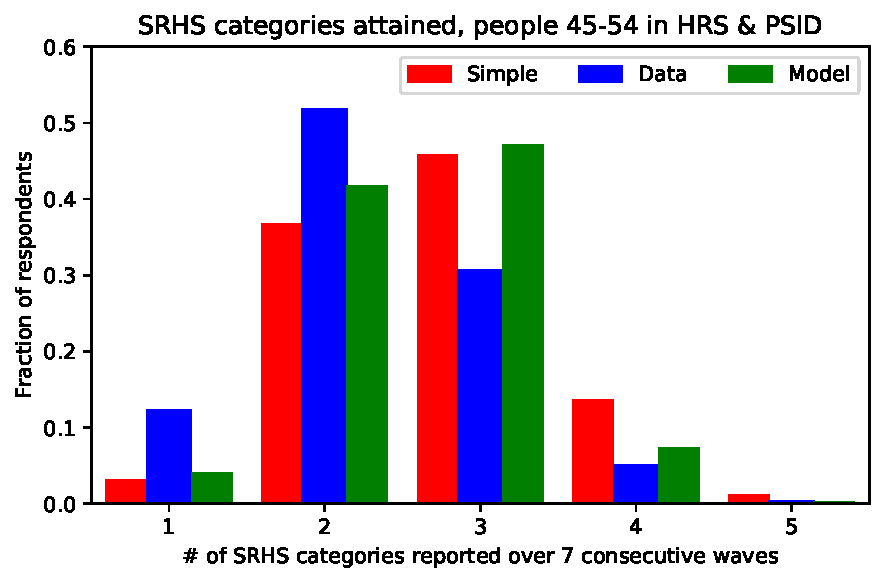
\includegraphics[width=\textwidth]{\FigsDir/TwoStudyOver23basicAllStateCount45to54.pdf}
		\caption{Ages 45-54 at baseline}\label{fig:StateCount45to54basic}
	\end{subfigure}
	~
	\begin{subfigure}[b]{0.48\textwidth}
		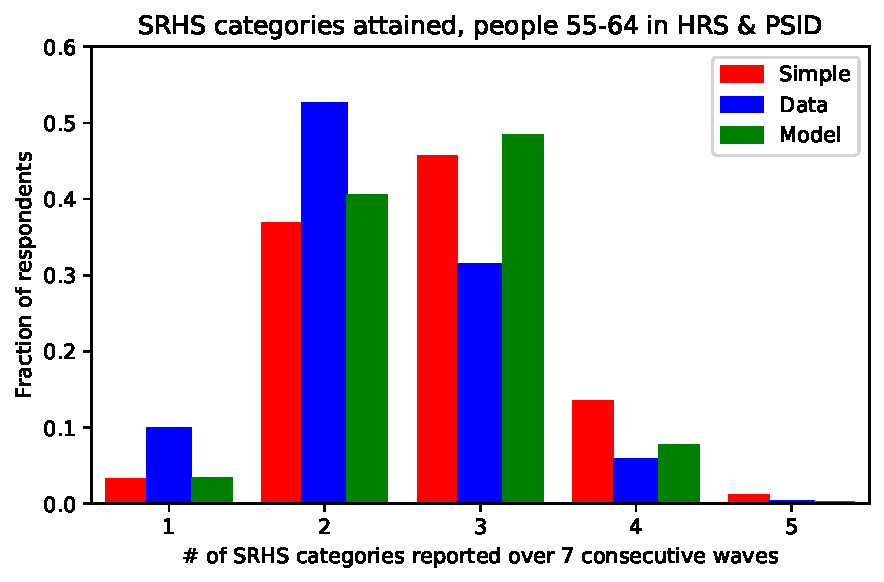
\includegraphics[width=\textwidth]{\FigsDir/TwoStudyOver23basicAllStateCount55to64.pdf}
		\caption{Ages 55-64 at baseline}\label{fig:StateCount55to64basic}
	\end{subfigure}
	
	
	\begin{subfigure}[b]{0.48\textwidth}
		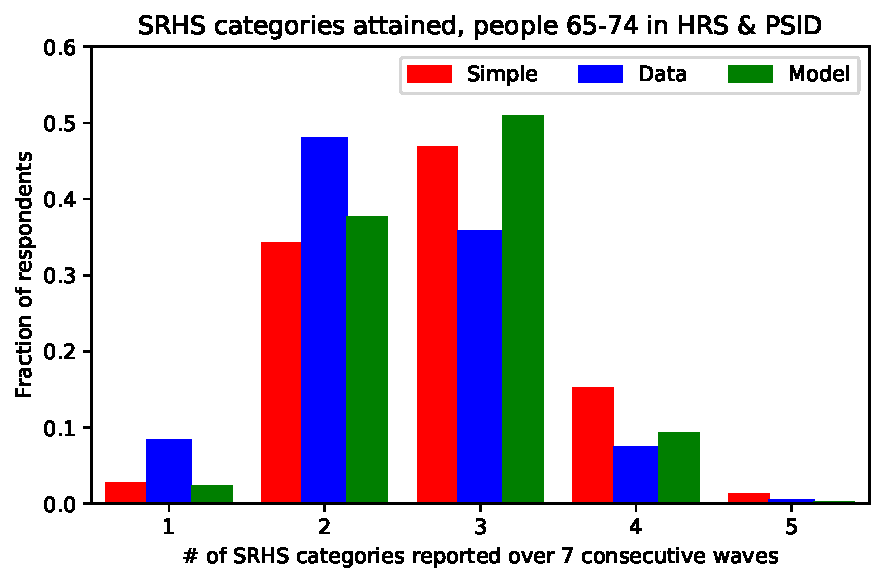
\includegraphics[width=\textwidth]{\FigsDir/TwoStudyOver23basicAllStateCount65to74.pdf}
		\caption{Ages 65-74 at baseline}\label{fig:StateCount65to74basic}
	\end{subfigure}
	~
	\begin{subfigure}[b]{0.48\textwidth}
		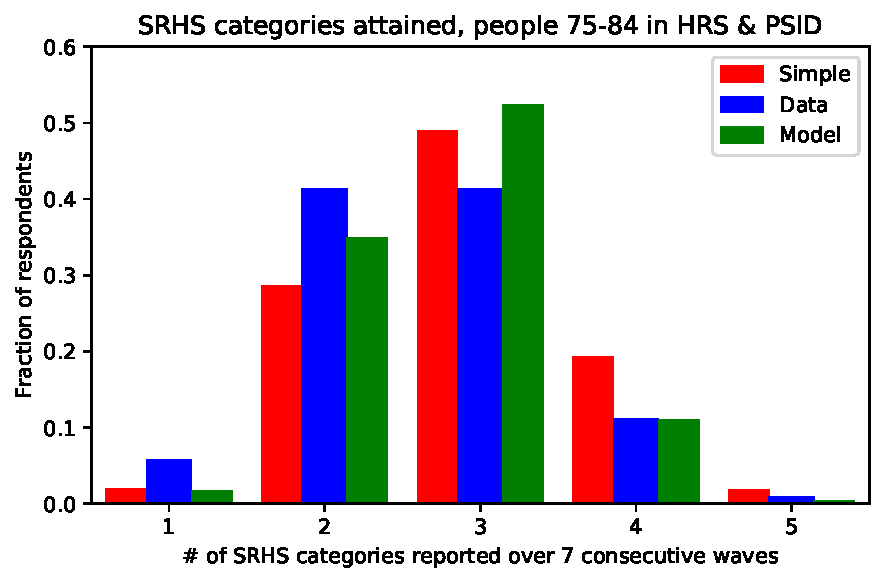
\includegraphics[width=\textwidth]{\FigsDir/TwoStudyOver23basicAllStateCount75to84.pdf}
		\caption{Ages 75-84 at baseline}\label{fig:StateCount75to84basic}
	\end{subfigure}
	\caption{Distribution of number of different health categories reported over 12 years (7 consecutive waves) using a balanced panel, model vs data vs simple dynamics. Basic model version assumes standard normal latent health shocks and no reporting error heterogeneity. Basic model has too many respondents who report three different SRHS categories over seven waves, and too few who report one or two.}\label{fig:StateCountTwoStudyBasic}
\end{figure}

The model presented in the paper includes heterogeneity in the magnitude of reporting errors, as well as mixed normal latent health shocks. A reader might reasonably wonder how a more basic model with simplified assumptions would perform, stripping these features. Table~\ref{tab:BasicTable} presents results for this basic model, specifying latent health shocks as standard normal and using only one reporting type (with $\varsigma=1$). The basic model fits conditional SRHS distributions fairly well, but is very inaccurate in predicting the fraction of respondents who consistently report bad health; Figure~\ref{fig:SRHSfreqUTwoStudybasic} provides the basic model analogue to Figure~\ref{fig:SRHSfreqUTwoStudy}, showing a bad fit in the rightmost column. Moreover, simulated basic model respondents visit too many different SRHS categories as compared to the data. Compare Figure~\ref{fig:StateCountTwoStudyBasic} here to Figure~\ref{fig:StateCountTwoStudy} in the main text, and note that the basic model's distribution is closer to the ``simple dynamics'' distribution than the data itself, predicting far too few respondents who report the same SRHS for seven waves straight.


\section{Additional Figures}\label{app:MoreFigs}

There are far more figures that demonstrate the latent health model's ability to reproduce SRHS dynamics, and that the traditional simple dynamics of SRHS used in the structural literature do \textit{not}, than can reasonably included be in the main paper text. This appendix includes many additional figures that were produced but excluded from the main paper out of considerations for paper length and readability.

First, Figure~\ref{fig:SRHScompare} provides a comparison of the distribution of SRHS by age and sex in the HRS and PSID, showing that the two surveys are comparable for their overlapping age range. Figure~\ref{fig:MortFitByAge} compares the estimated model's predicted mortality rate by age and sex to the observed rate in the data as well as the values from the Social Security Administration's mortality tables for 2013; the differences among the trends are often imperceptible, providing some basic validation of the dataset as a representative sample of the U.S.\ population.

In the main paper, Figure~\ref{fig:NaiveTransVG} shows that the simple health dynamics used in almost all structural models do not accurately fit the empirical distribution of SRHS (conditional on reporting ``very good'' health at baseline) several waves in the future. I repeat the same exercise for all five categorical health states in Figures~\ref{fig:NaiveTransPR}-\ref{fig:NaiveTransEX}, comparing predictions from simple dynamics to the HRS and PSID data up to sixteen years ahead. Simple dynamics generate an extremely poor fit to the data.

In contrast, the latent health model accurately matches the empirical distribution of SRHS (conditional on age and health in the baseline period) far into the future. Figures~\ref{fig:ModelTransPR}-\ref{fig:ModelTransEX} plot the distribution of SRHS one to eight waves ahead, comparing the estimated model's predictions to observations from the HRS and PSID. The largest differences between the model and data occur for younger respondents (under 40) initially observed in poor health, and older respondents (75+) in very good or excellent health. In each case, there are relatively few relevant observations on which to discipline the model. Note that the model fit deteriorates completely when making predictions about very old ages (95 and beyond), as there are extremely few observations at all.

In the main text of the paper, Figure~\ref{fig:SRHSfreqUTwoStudy} shows that the model accurately predicts the frequency of bad health (reporting poor or fair SRHS) over the next six waves conditional on bad health at baseline. Figure~\ref{fig:SRHSfreqHTwoStudy} below shows that the model also matches the frequency distribution conditional on good health at baseline as well. However, the simple dynamics of SRHS do not generate such a bad fit as they do when starting from bad health, so the latent health model only provides a modest improvement here.

Finally, Figure~\ref{fig:ChangeSRHS} plots the model-predicted probability of reporting two different SRHS categories if asked twice in the same wave. Other than younger respondents in poor or fair health (of whom there are relatively few), the model predicts a probability of changing answers that is fairly constant with respect to age and health.

\begin{figure}
	\centering
	\begin{subfigure}[b]{0.48\textwidth}
		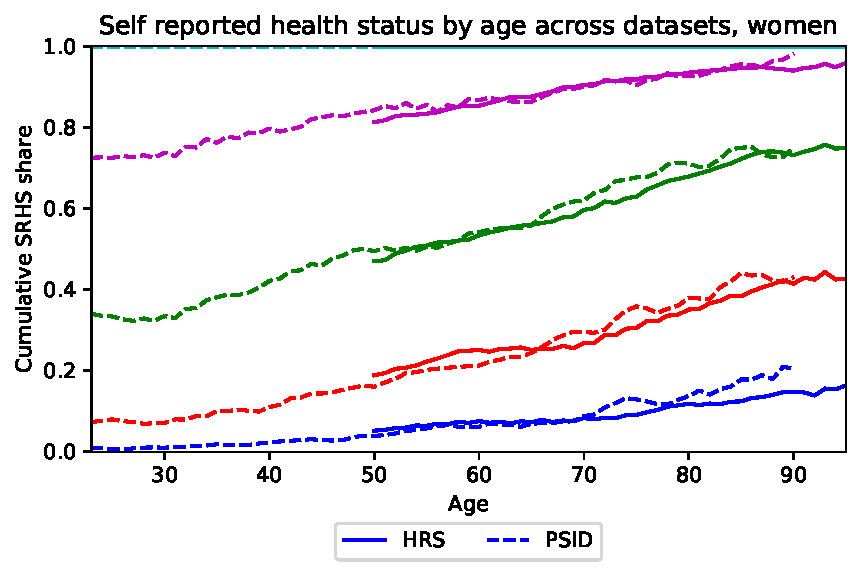
\includegraphics[width=\textwidth]{\FigsDir/TwoStudySRHSaWomen.pdf}
		\caption{HRS \& PSID women}\label{fig:SRHScompareWomen}
	\end{subfigure}
	~
	\begin{subfigure}[b]{0.48\textwidth}
		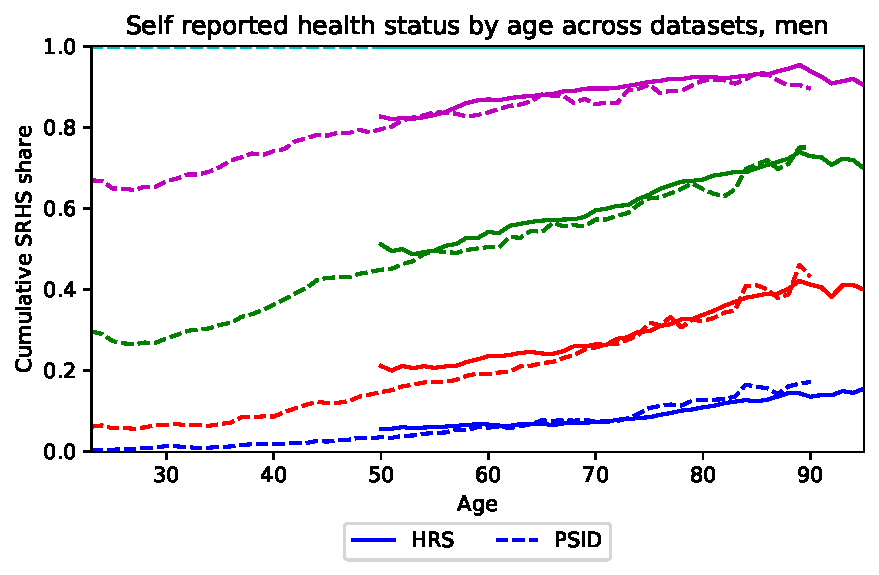
\includegraphics[width=\textwidth]{\FigsDir/TwoStudySRHSaMen.pdf}
		\caption{HRS \& PSID men}\label{fig:SRHScompareMen}
	\end{subfigure}
	\caption{Distribution of SRHS by age in the HRS and PSID data.}\label{fig:SRHScompare}
\end{figure}

\begin{figure}
	\centering
	\begin{subfigure}[b]{0.48\textwidth}
		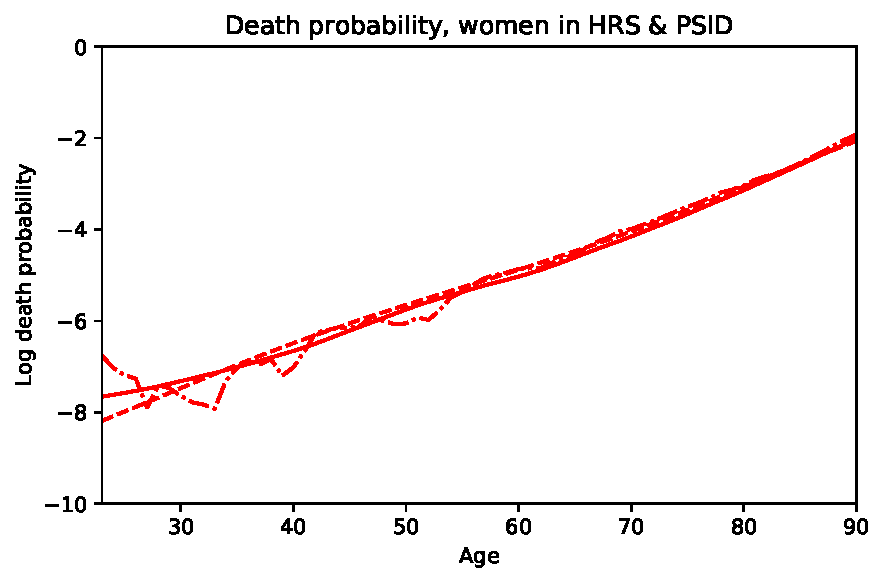
\includegraphics[width=\textwidth]{\FigsDir/TwoStudyOver23WomenMortByAge.pdf}
		\caption{HRS \& PSID women}\label{fig:MEPSwomenMortAge}
	\end{subfigure}
	~
	\centering
	\begin{subfigure}[b]{0.48\textwidth}
		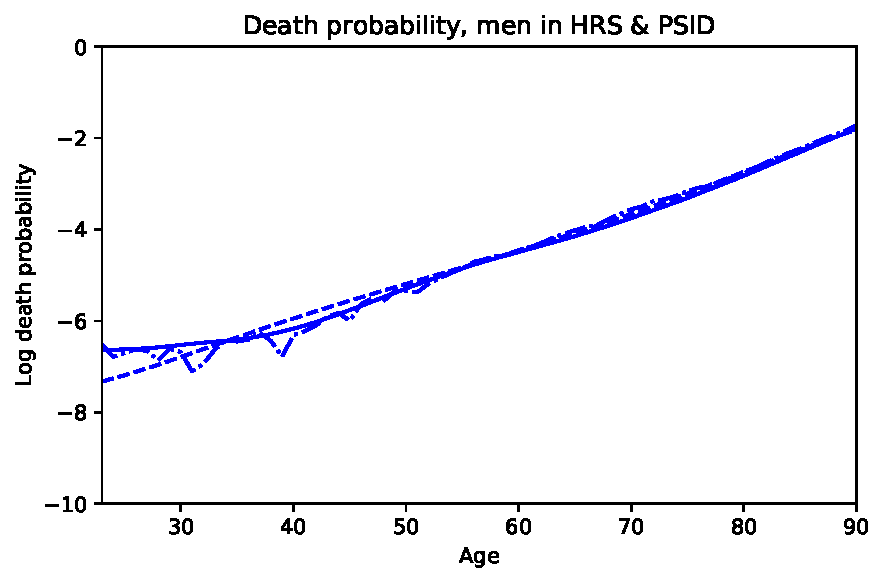
\includegraphics[width=\textwidth]{\FigsDir/TwoStudyOver23MenMortByAge.pdf}
		\caption{HRS \& PSID men}\label{fig:TwoStudyMenMortAge}
	\end{subfigure}
	\caption{Mortality by age, SSA table (solid) vs data (dash-dot) vs estimated model.} \label{fig:MortFitByAge}
\end{figure}



\begin{figure}
	\centering
	\begin{subfigure}[b]{0.48\textwidth}
		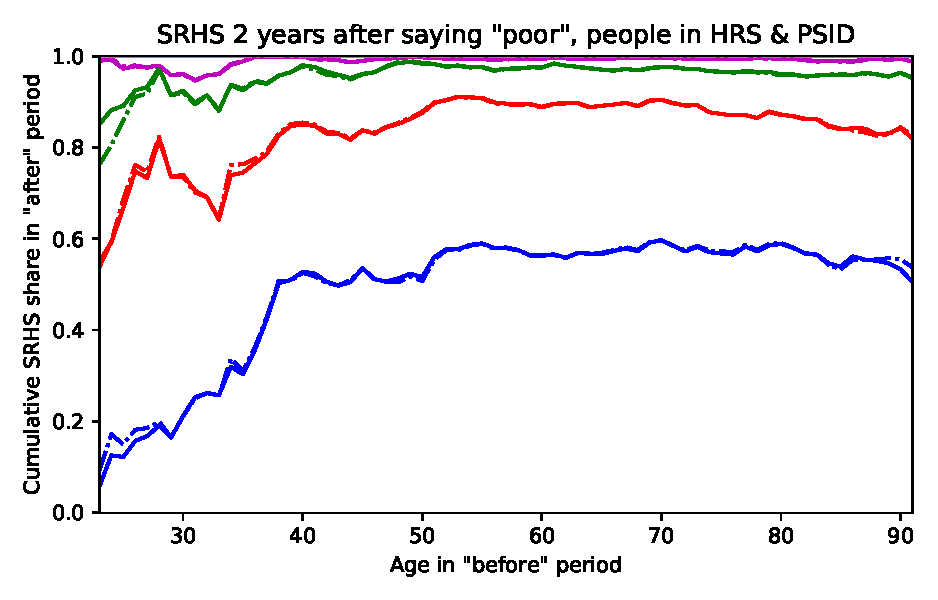
\includegraphics[width=\textwidth]{\FigsDir/TwoStudyOver23AllTransH1T2naiveNoLeg.pdf}
		\caption{One wave ahead}\label{fig:Naive1AheadPoor}
	\end{subfigure}
	~
	\begin{subfigure}[b]{0.48\textwidth}
		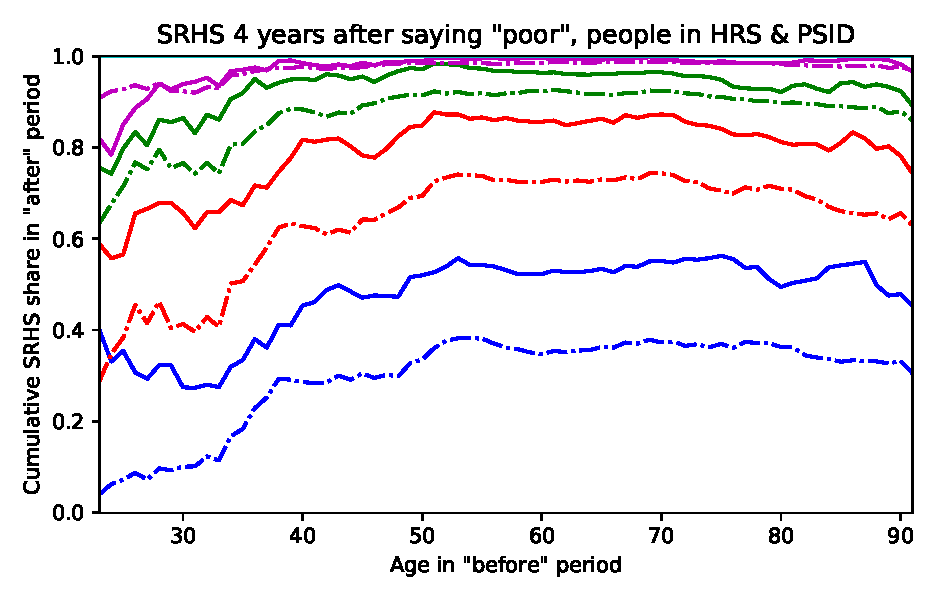
\includegraphics[width=\textwidth]{\FigsDir/TwoStudyOver23AllTransH1T4naiveNoLeg.pdf}
		\caption{Two waves ahead}\label{fig:Naive2AheadPoor}
	\end{subfigure}
	
	\begin{subfigure}[b]{0.48\textwidth}
		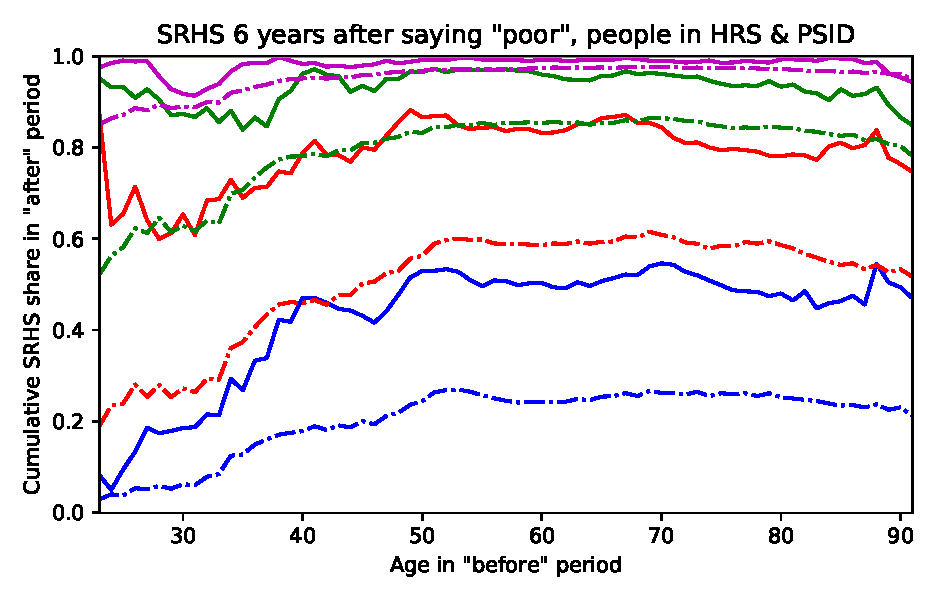
\includegraphics[width=\textwidth]{\FigsDir/TwoStudyOver23AllTransH1T6naiveNoLeg.pdf}
		\caption{Three waves ahead}\label{fig:Naive3AheadPoor}
	\end{subfigure}
	~
	\begin{subfigure}[b]{0.48\textwidth}
		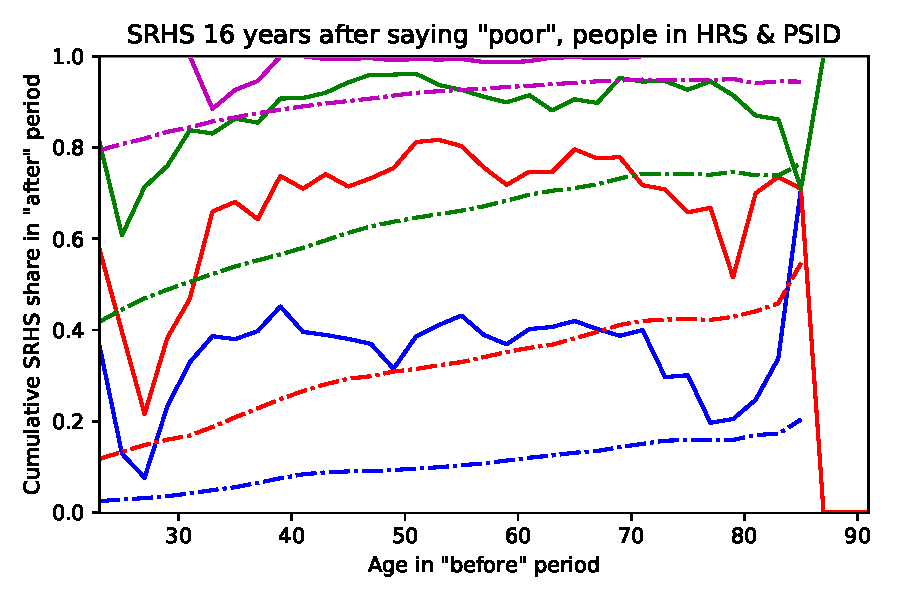
\includegraphics[width=\textwidth]{\FigsDir/TwoStudyOver23AllTransH1T8naiveNoLeg.pdf}
		\caption{Four waves ahead}\label{fig:Naive4AheadPoor}
	\end{subfigure}
	
	\begin{subfigure}[b]{0.48\textwidth}
		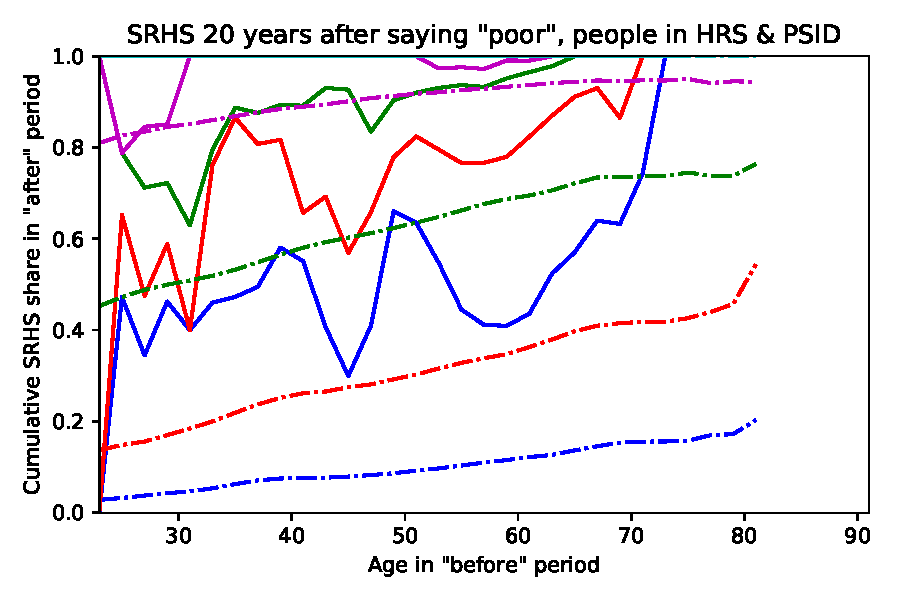
\includegraphics[width=\textwidth]{\FigsDir/TwoStudyOver23AllTransH1T10naiveNoLeg.pdf}
		\caption{Five waves ahead}\label{fig:Naive5AheadPoor}
	\end{subfigure}
	~
	\begin{subfigure}[b]{0.48\textwidth}
		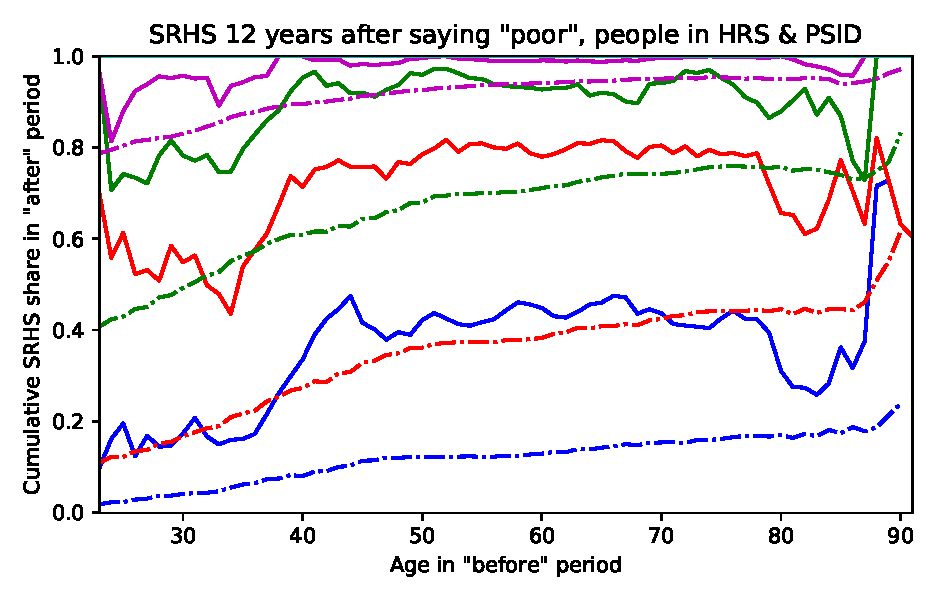
\includegraphics[width=\textwidth]{\FigsDir/TwoStudyOver23AllTransH1T12naiveNoLeg.pdf}
		\caption{Six waves ahead}\label{fig:Naive6AheadPoor}
	\end{subfigure}
	
	\begin{subfigure}[b]{0.48\textwidth}
		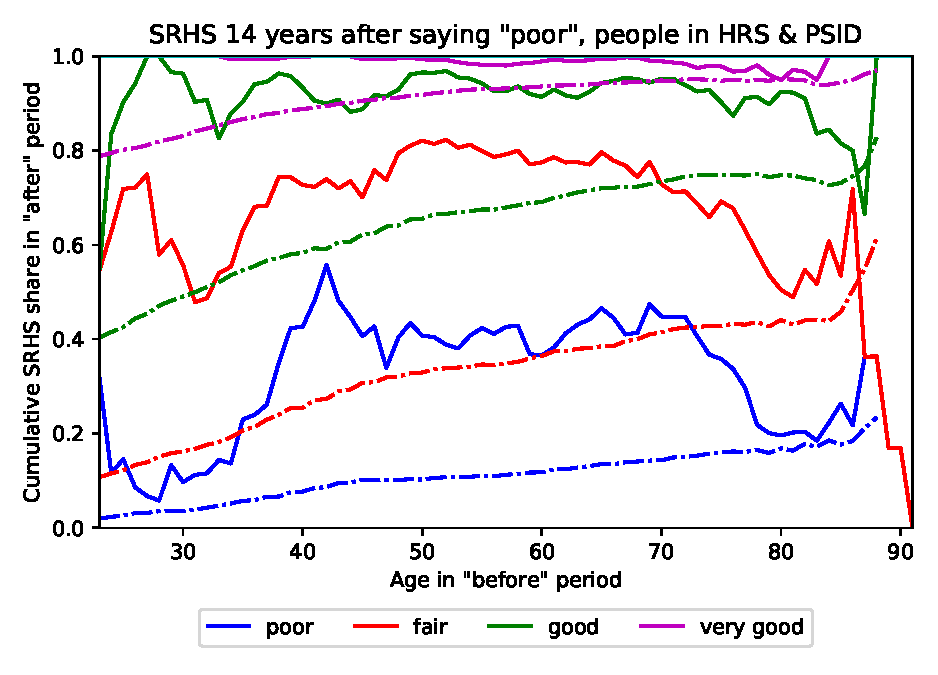
\includegraphics[width=\textwidth]{\FigsDir/TwoStudyOver23AllTransH1T14naive.pdf}
		\caption{Seven waves ahead}\label{fig:Naive7AheadPoor}
	\end{subfigure}
	~
	\begin{subfigure}[b]{0.48\textwidth}
		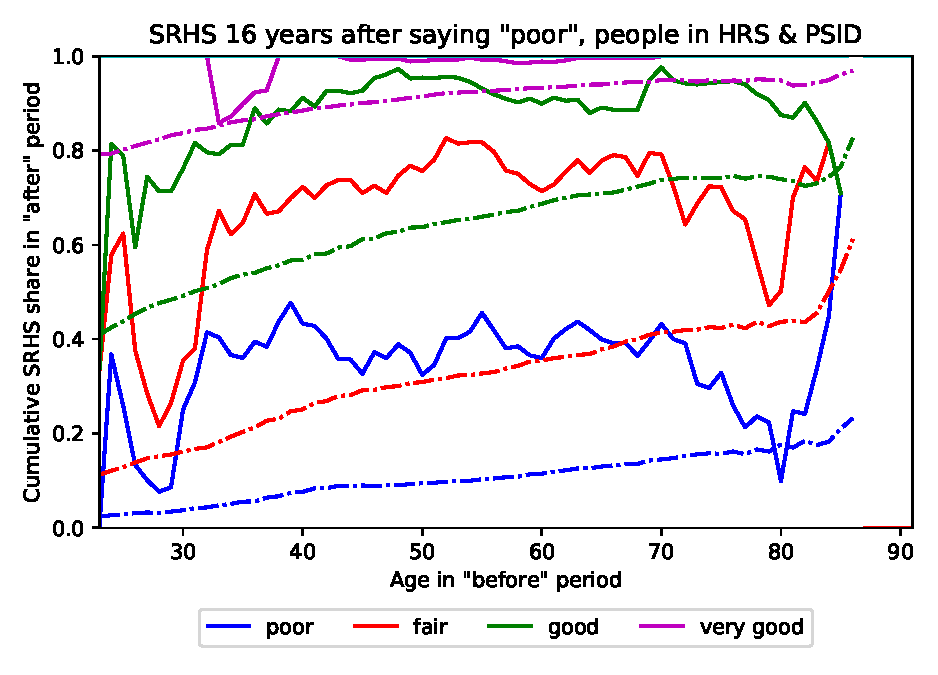
\includegraphics[width=\textwidth]{\FigsDir/TwoStudyOver23AllTransH1T16naive.pdf}
		\caption{Eight waves ahead}\label{fig:Naive8AheadPoor}
	\end{subfigure}
	\caption{Cumulative distribution of SRHS by age conditional on reporting ``poor'' health in the baseline period in the PSID \& HRS data (solid) vs simple dynamics (dash-dot).}\label{fig:NaiveTransPR}
\end{figure}


\begin{figure}
	\centering
	\begin{subfigure}[b]{0.48\textwidth}
		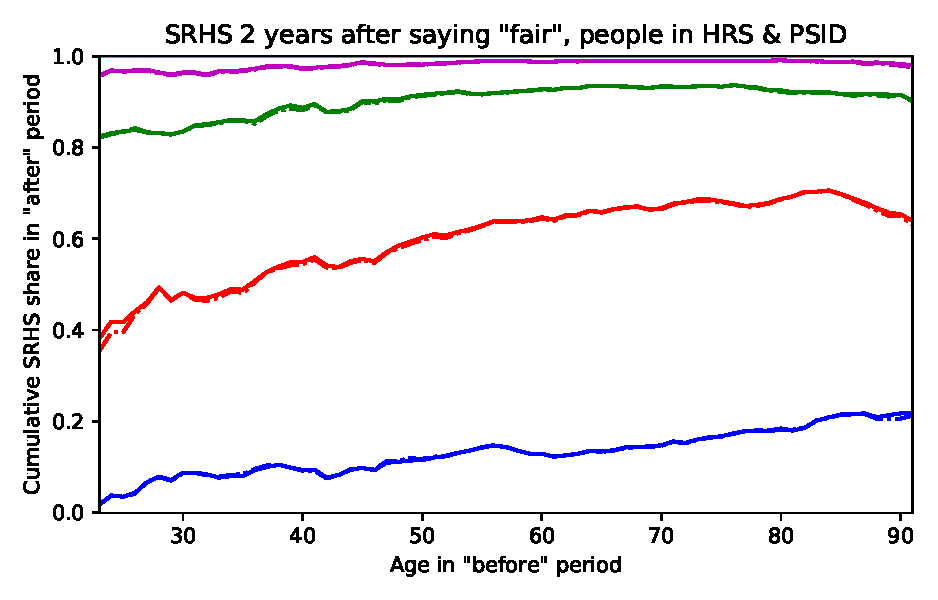
\includegraphics[width=\textwidth]{\FigsDir/TwoStudyOver23AllTransH2T2naiveNoLeg.pdf}
		\caption{One wave ahead}\label{fig:Naive1AheadFair}
	\end{subfigure}
	~
	\begin{subfigure}[b]{0.48\textwidth}
		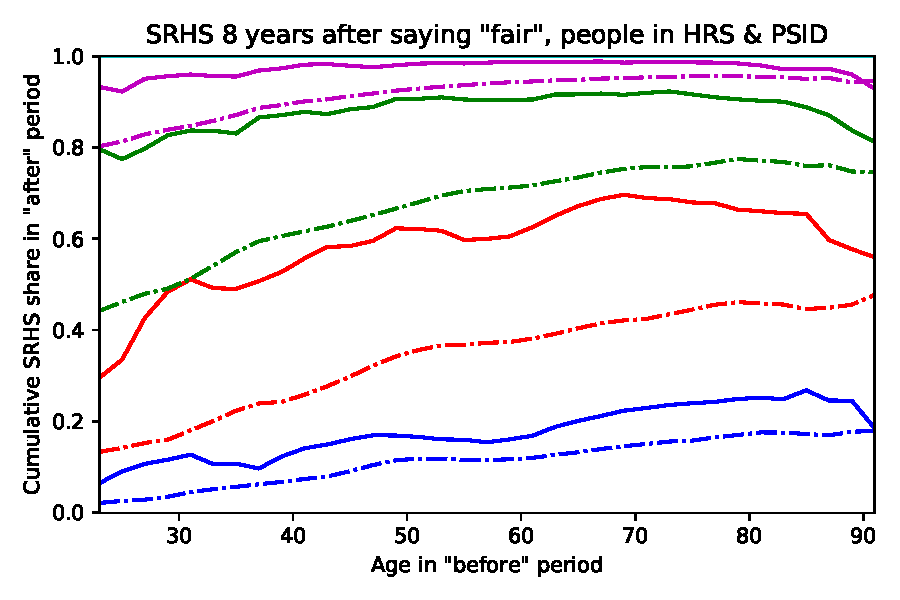
\includegraphics[width=\textwidth]{\FigsDir/TwoStudyOver23AllTransH2T4naiveNoLeg.pdf}
		\caption{Two waves ahead}\label{fig:Naive2AheadFair}
	\end{subfigure}
	
	\begin{subfigure}[b]{0.48\textwidth}
		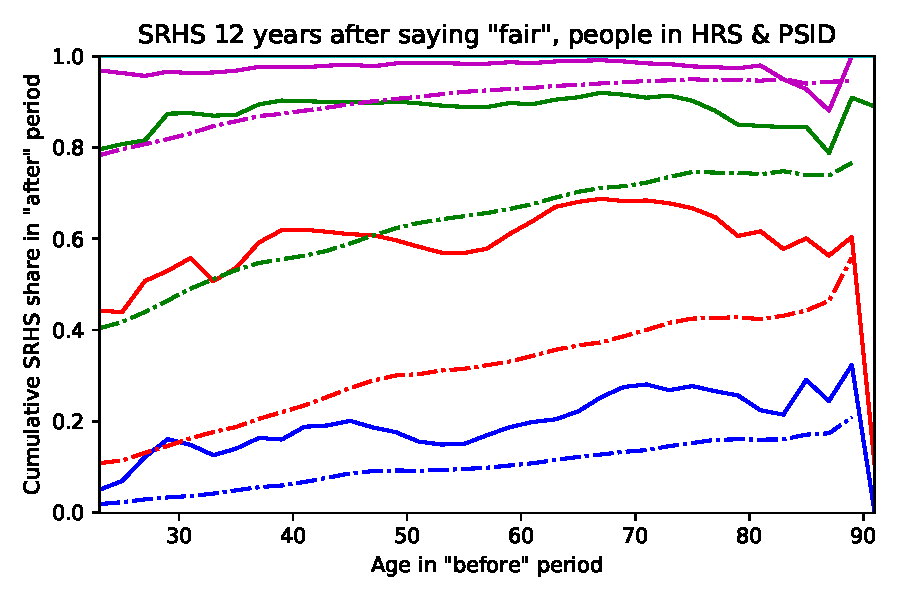
\includegraphics[width=\textwidth]{\FigsDir/TwoStudyOver23AllTransH2T6naiveNoLeg.pdf}
		\caption{Three waves ahead}\label{fig:Naive3AheadFair}
	\end{subfigure}
	~
	\begin{subfigure}[b]{0.48\textwidth}
		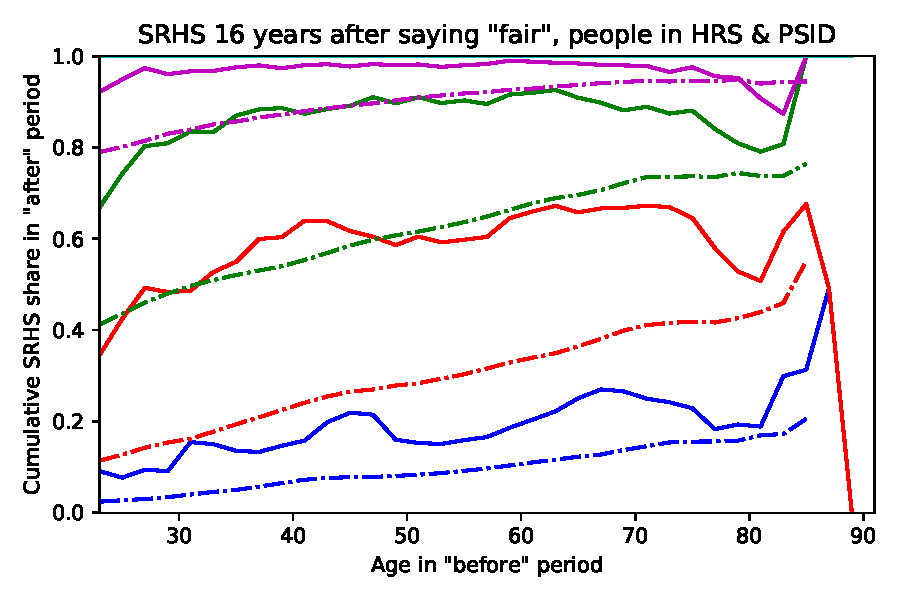
\includegraphics[width=\textwidth]{\FigsDir/TwoStudyOver23AllTransH2T8naiveNoLeg.pdf}
		\caption{Four waves ahead}\label{fig:Naive4AheadFair}
	\end{subfigure}
	
	\begin{subfigure}[b]{0.48\textwidth}
		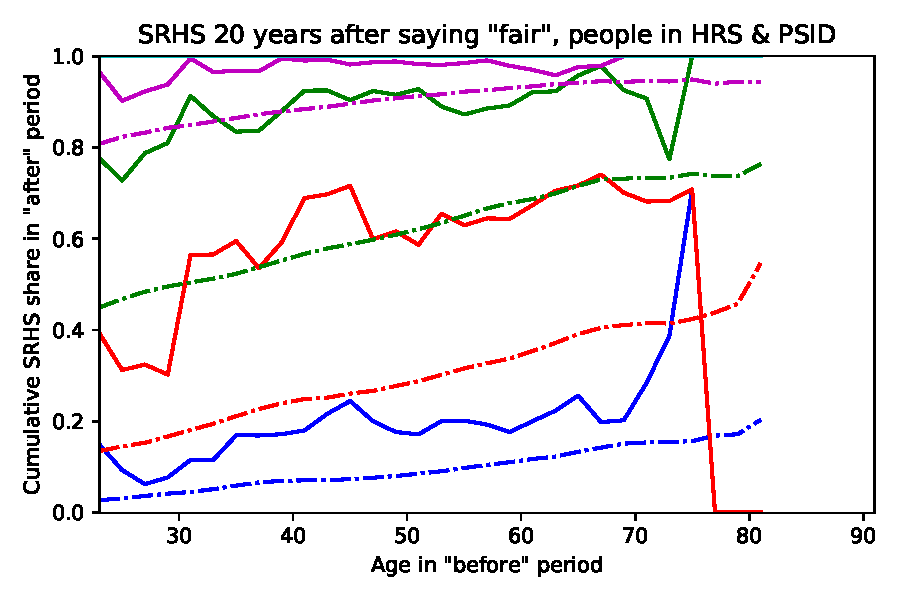
\includegraphics[width=\textwidth]{\FigsDir/TwoStudyOver23AllTransH2T10naiveNoLeg.pdf}
		\caption{Five waves ahead}\label{fig:Naive5AheadFair}
	\end{subfigure}
	~
	\begin{subfigure}[b]{0.48\textwidth}
		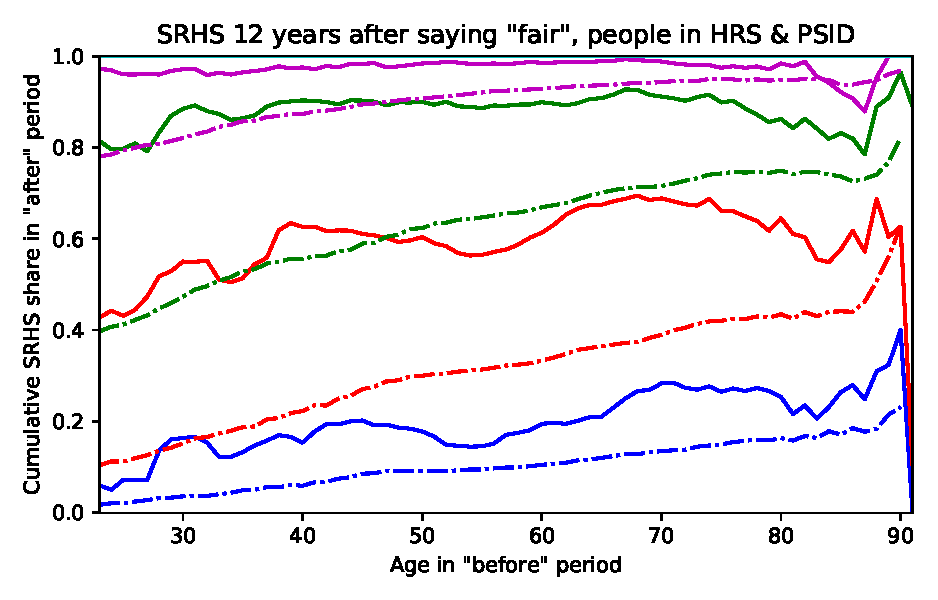
\includegraphics[width=\textwidth]{\FigsDir/TwoStudyOver23AllTransH2T12naiveNoLeg.pdf}
		\caption{Six waves ahead}\label{fig:Naive6AheadFair}
	\end{subfigure}
	
	\begin{subfigure}[b]{0.48\textwidth}
		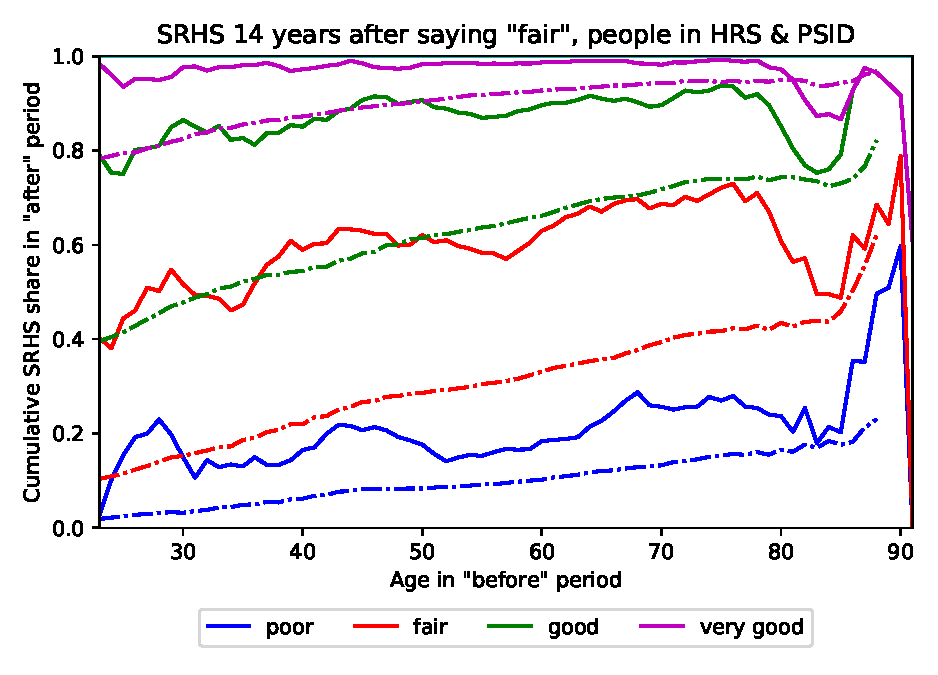
\includegraphics[width=\textwidth]{\FigsDir/TwoStudyOver23AllTransH2T14naive.pdf}
		\caption{Seven waves ahead}\label{fig:Naive7AheadFair}
	\end{subfigure}
	~
	\begin{subfigure}[b]{0.48\textwidth}
		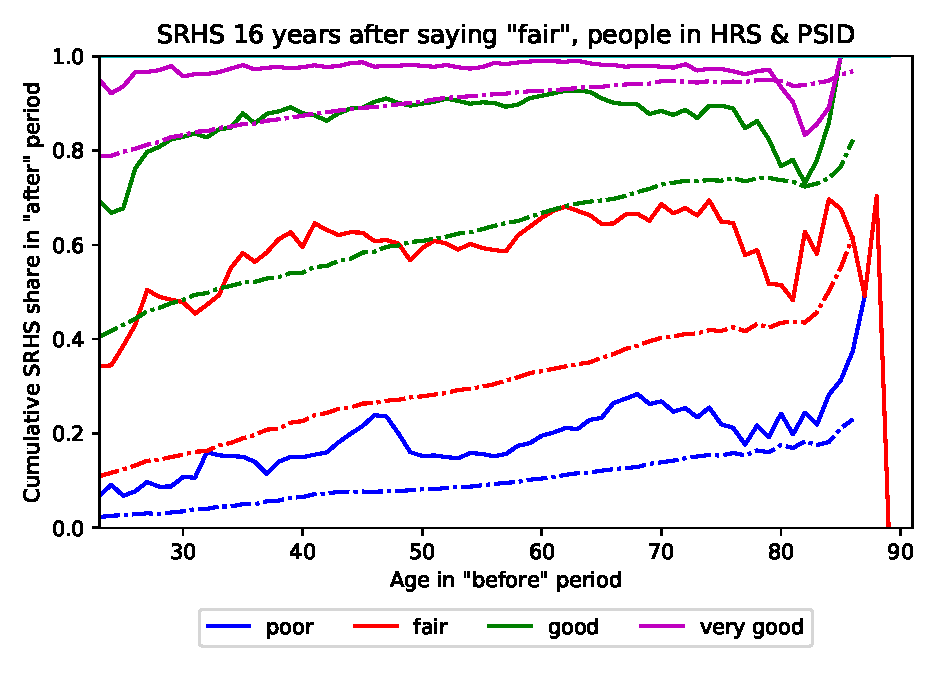
\includegraphics[width=\textwidth]{\FigsDir/TwoStudyOver23AllTransH2T16naive.pdf}
		\caption{Eight waves ahead}\label{fig:Naive8AheadFair}
	\end{subfigure}
	\caption{Cumulative distribution of SRHS by age conditional on reporting ``fair'' health in the baseline period in the PSID \& HRS data (solid) vs simple dynamics (dash-dot).}\label{fig:NaiveTransFR}
\end{figure}


\begin{figure}
	\centering
	\begin{subfigure}[b]{0.48\textwidth}
		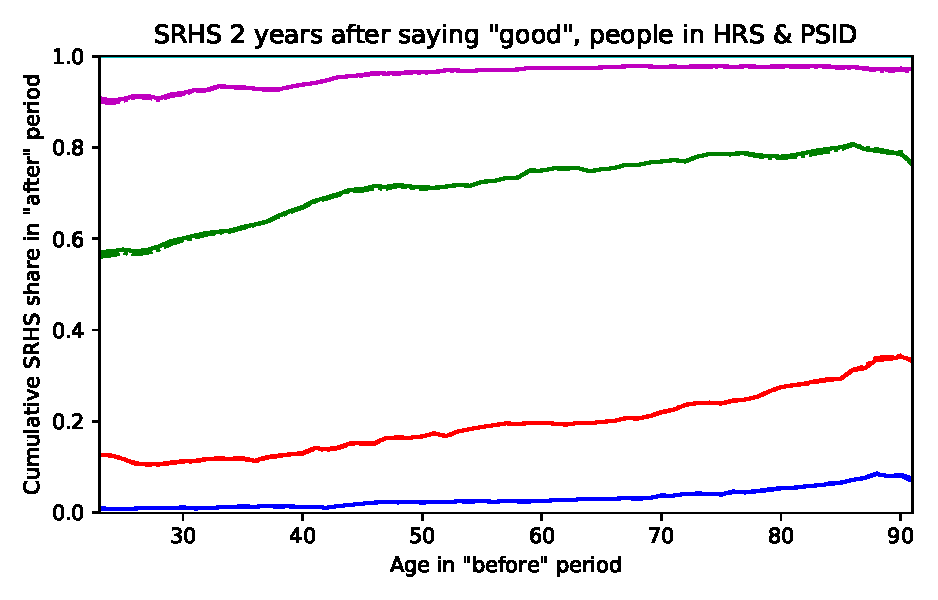
\includegraphics[width=\textwidth]{\FigsDir/TwoStudyOver23AllTransH3T2naiveNoLeg.pdf}
		\caption{One wave ahead}\label{fig:Naive1AheadGood}
	\end{subfigure}
	~
	\begin{subfigure}[b]{0.48\textwidth}
		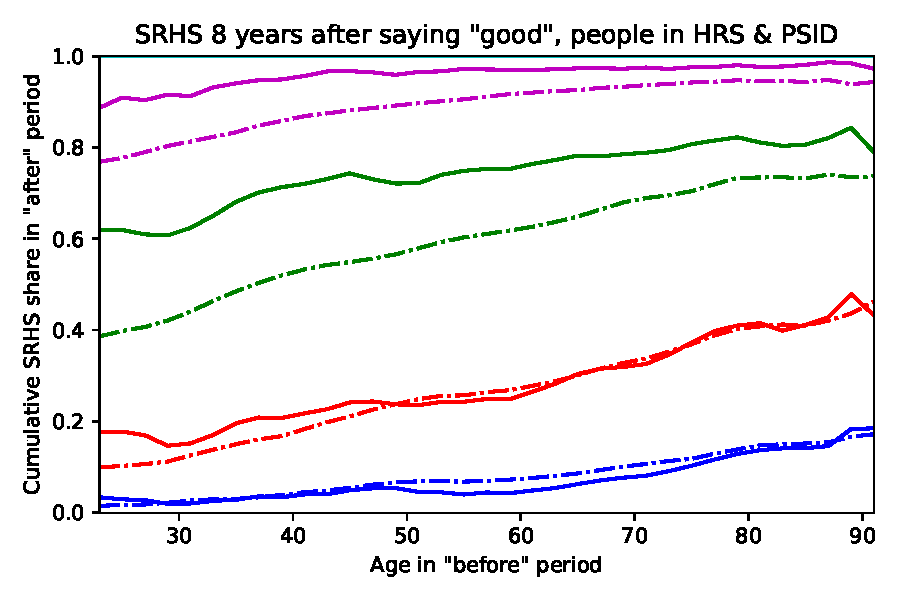
\includegraphics[width=\textwidth]{\FigsDir/TwoStudyOver23AllTransH3T4naiveNoLeg.pdf}
		\caption{Two waves ahead}\label{fig:Naive2AheadGood}
	\end{subfigure}
	
	\begin{subfigure}[b]{0.48\textwidth}
		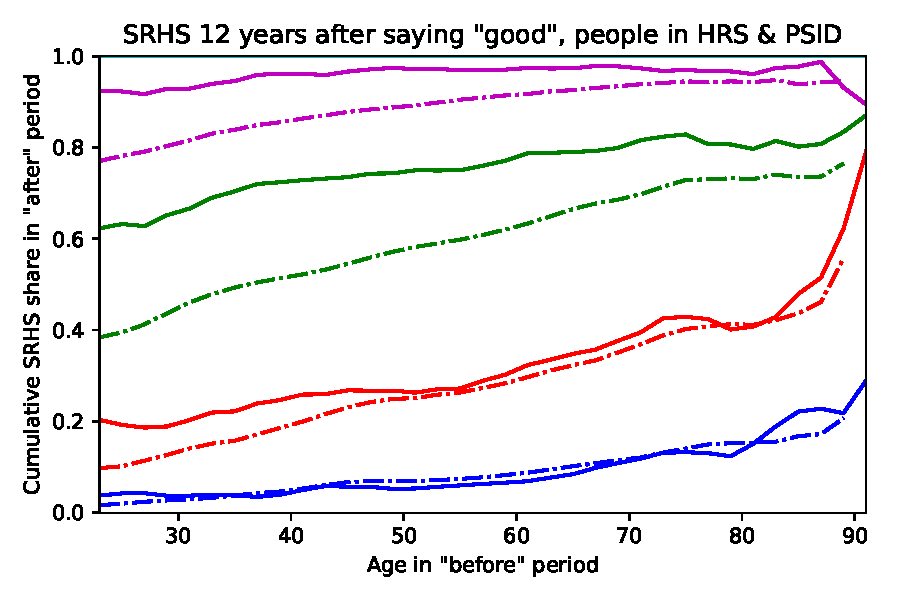
\includegraphics[width=\textwidth]{\FigsDir/TwoStudyOver23AllTransH3T6naiveNoLeg.pdf}
		\caption{Three waves ahead}\label{fig:Naive3AheadGood}
	\end{subfigure}
	~
	\begin{subfigure}[b]{0.48\textwidth}
		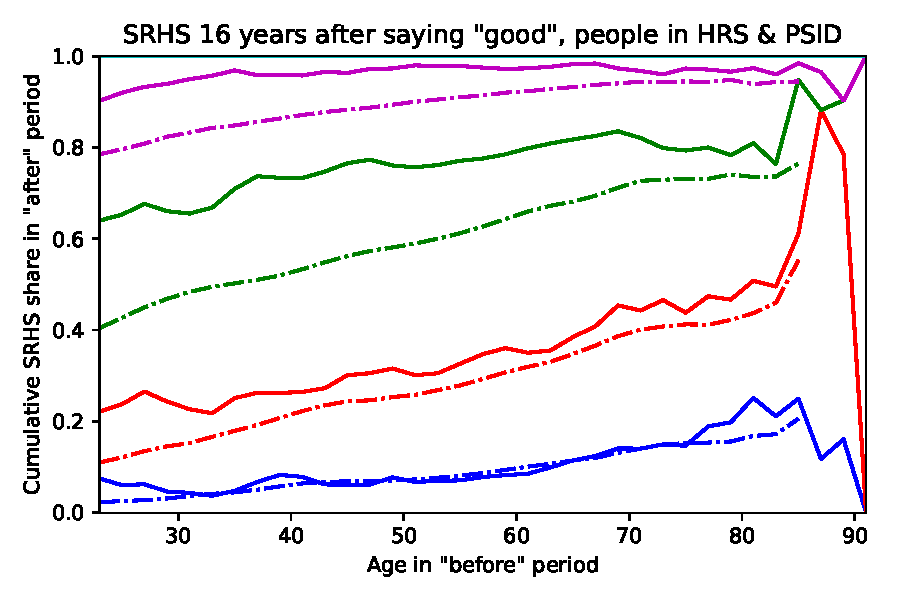
\includegraphics[width=\textwidth]{\FigsDir/TwoStudyOver23AllTransH3T8naiveNoLeg.pdf}
		\caption{Four waves ahead}\label{fig:Naive4AheadGood}
	\end{subfigure}
	
	\begin{subfigure}[b]{0.48\textwidth}
		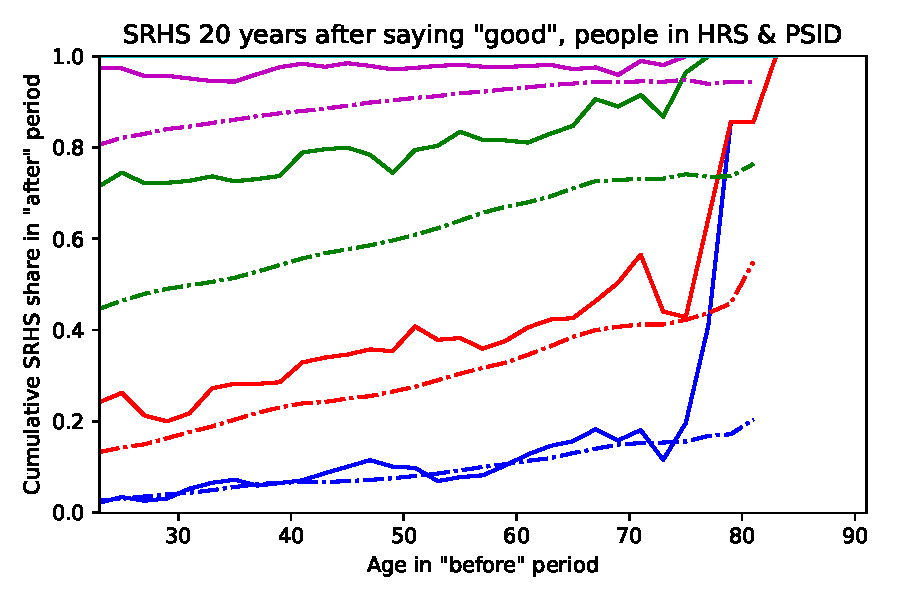
\includegraphics[width=\textwidth]{\FigsDir/TwoStudyOver23AllTransH3T10naiveNoLeg.pdf}
		\caption{Five waves ahead}\label{fig:Naive5AheadGood}
	\end{subfigure}
	~
	\begin{subfigure}[b]{0.48\textwidth}
		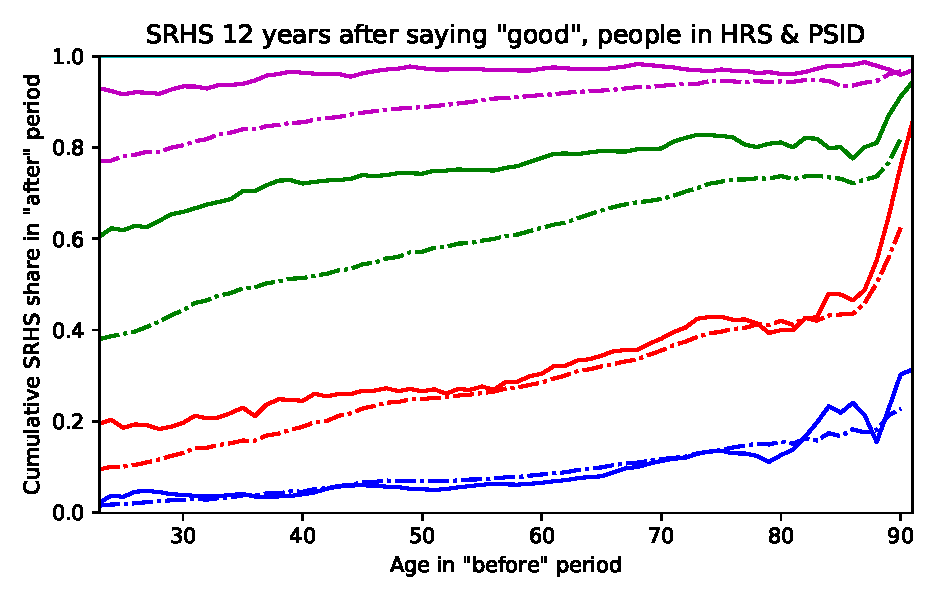
\includegraphics[width=\textwidth]{\FigsDir/TwoStudyOver23AllTransH3T12naiveNoLeg.pdf}
		\caption{Six waves ahead}\label{fig:Naive6AheadGood}
	\end{subfigure}
	
	\begin{subfigure}[b]{0.48\textwidth}
		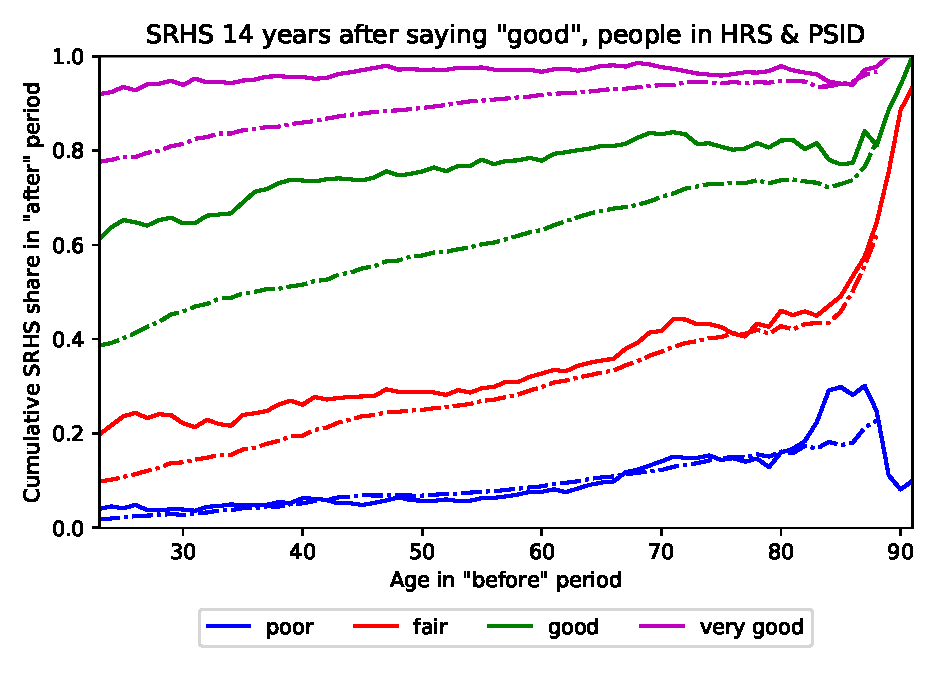
\includegraphics[width=\textwidth]{\FigsDir/TwoStudyOver23AllTransH3T14naive.pdf}
		\caption{Seven waves ahead}\label{fig:Naive7AheadGood}
	\end{subfigure}
	~
	\begin{subfigure}[b]{0.48\textwidth}
		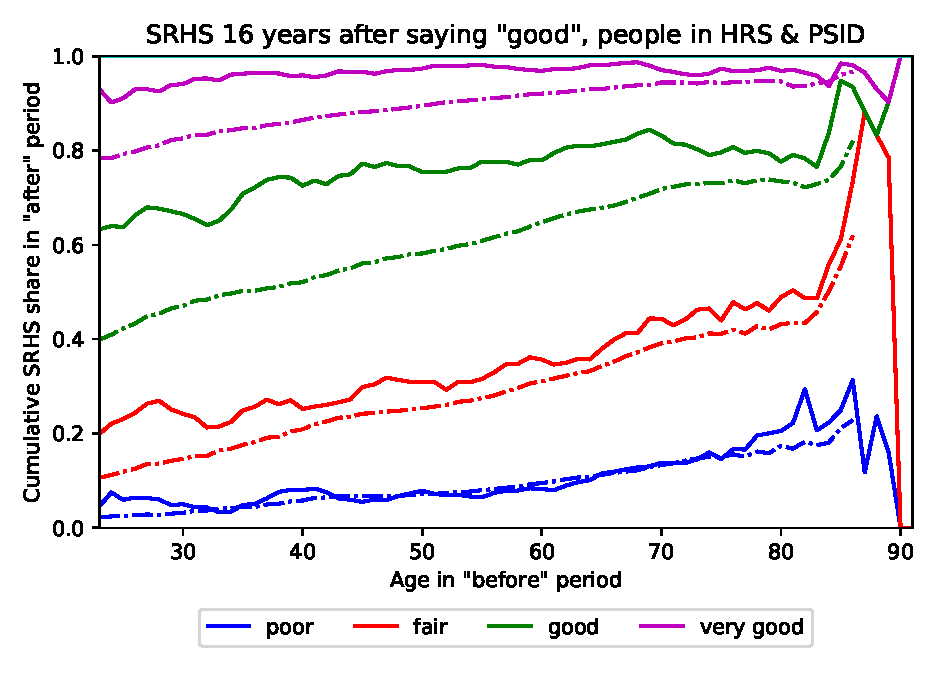
\includegraphics[width=\textwidth]{\FigsDir/TwoStudyOver23AllTransH3T16naive.pdf}
		\caption{Eight waves ahead}\label{fig:Naive8AheadGood}
	\end{subfigure}
	\caption{Cumulative distribution of SRHS by age conditional on reporting ``good'' health in the baseline period in the PSID \& HRS data (solid) vs simple dynamics (dash-dot).}\label{fig:NaiveTransGD}
\end{figure}


\begin{figure}
	\centering
	\begin{subfigure}[b]{0.48\textwidth}
		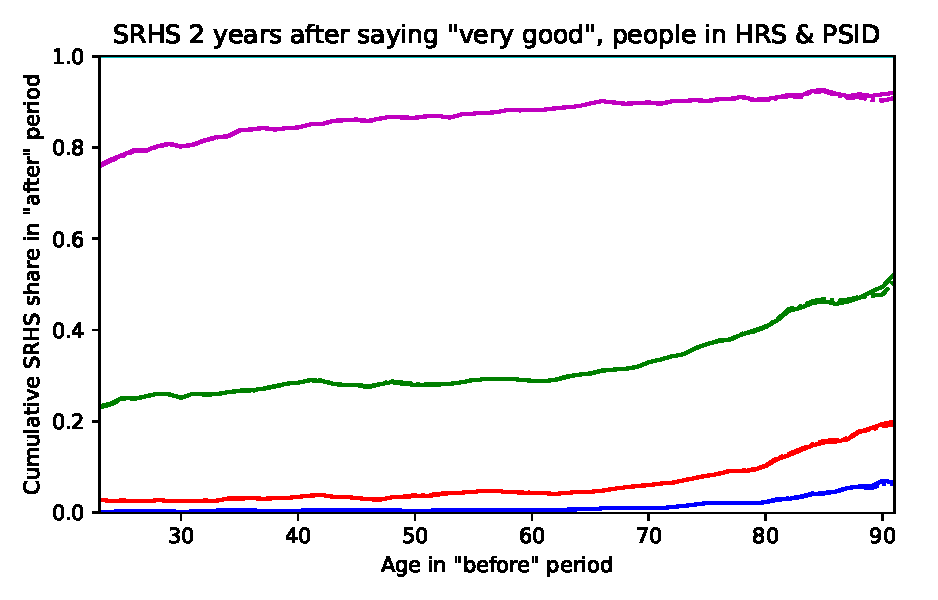
\includegraphics[width=\textwidth]{\FigsDir/TwoStudyOver23AllTransH4T2naiveNoLeg.pdf}
		\caption{One wave ahead}\label{fig:Naive1AheadVeryGood}
	\end{subfigure}
	~
	\begin{subfigure}[b]{0.48\textwidth}
		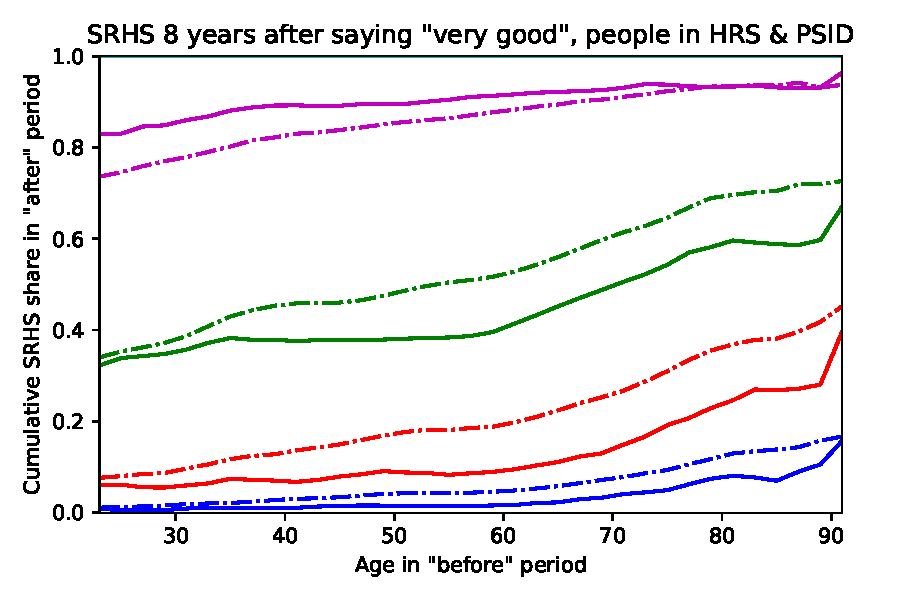
\includegraphics[width=\textwidth]{\FigsDir/TwoStudyOver23AllTransH4T4naiveNoLeg.pdf}
		\caption{Two waves ahead}\label{fig:Naive2AheadVeryGood}
	\end{subfigure}
	
	\begin{subfigure}[b]{0.48\textwidth}
		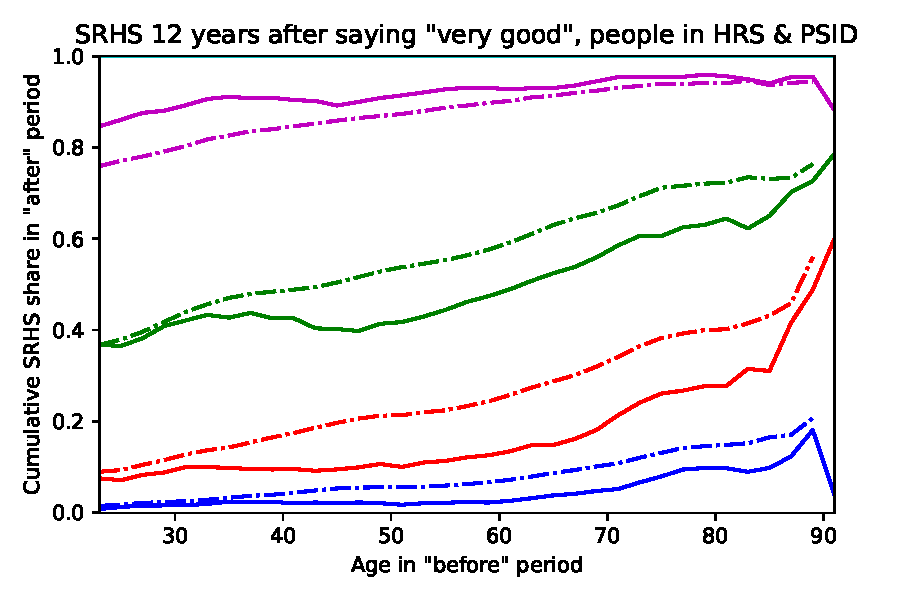
\includegraphics[width=\textwidth]{\FigsDir/TwoStudyOver23AllTransH4T6naiveNoLeg.pdf}
		\caption{Three waves ahead}\label{fig:Naive3AheadVeryGood}
	\end{subfigure}
	~
	\begin{subfigure}[b]{0.48\textwidth}
		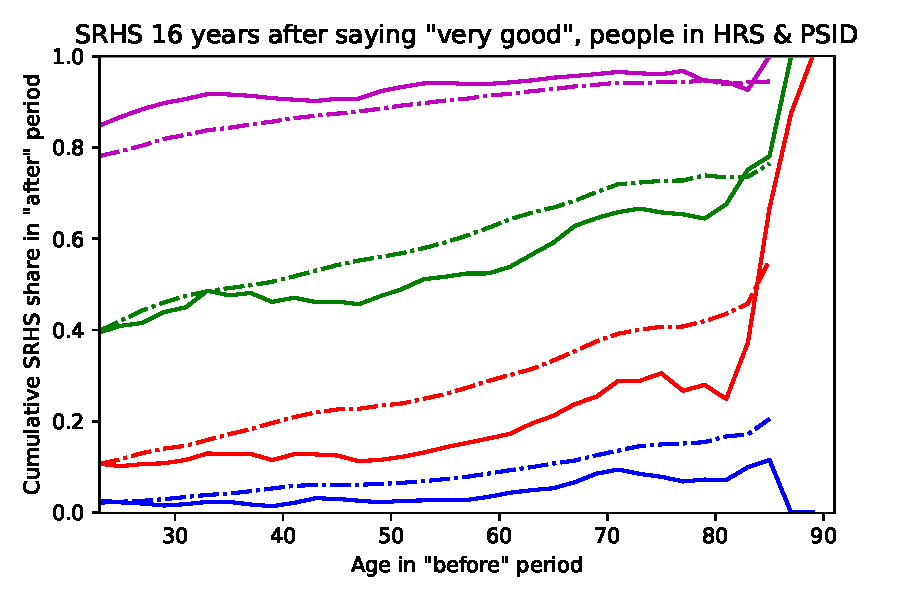
\includegraphics[width=\textwidth]{\FigsDir/TwoStudyOver23AllTransH4T8naiveNoLeg.pdf}
		\caption{Four waves ahead}\label{fig:Naive4AheadVeryGood}
	\end{subfigure}
	
	\begin{subfigure}[b]{0.48\textwidth}
		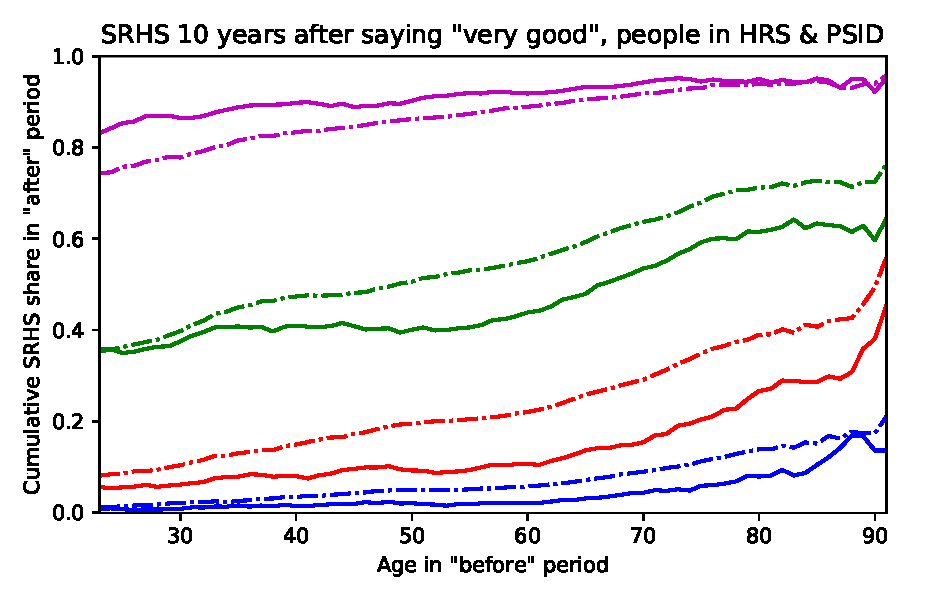
\includegraphics[width=\textwidth]{\FigsDir/TwoStudyOver23AllTransH4T10naiveNoLeg.pdf}
		\caption{Five waves ahead}\label{fig:Naive5AheadVeryGood}
	\end{subfigure}
	~
	\begin{subfigure}[b]{0.48\textwidth}
		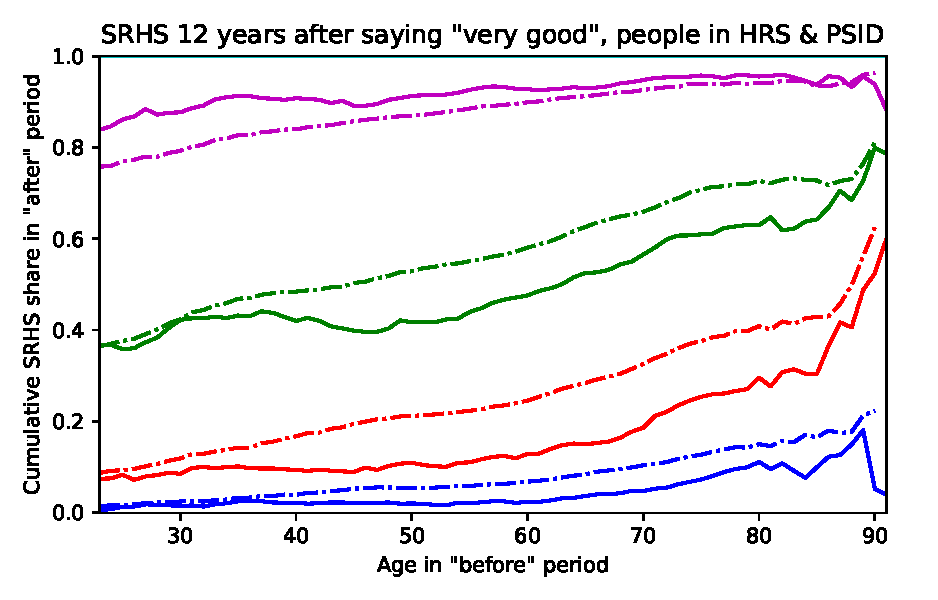
\includegraphics[width=\textwidth]{\FigsDir/TwoStudyOver23AllTransH4T12naiveNoLeg.pdf}
		\caption{Six waves ahead}\label{fig:Naive6AheadVeryGood}
	\end{subfigure}
	
	\begin{subfigure}[b]{0.48\textwidth}
		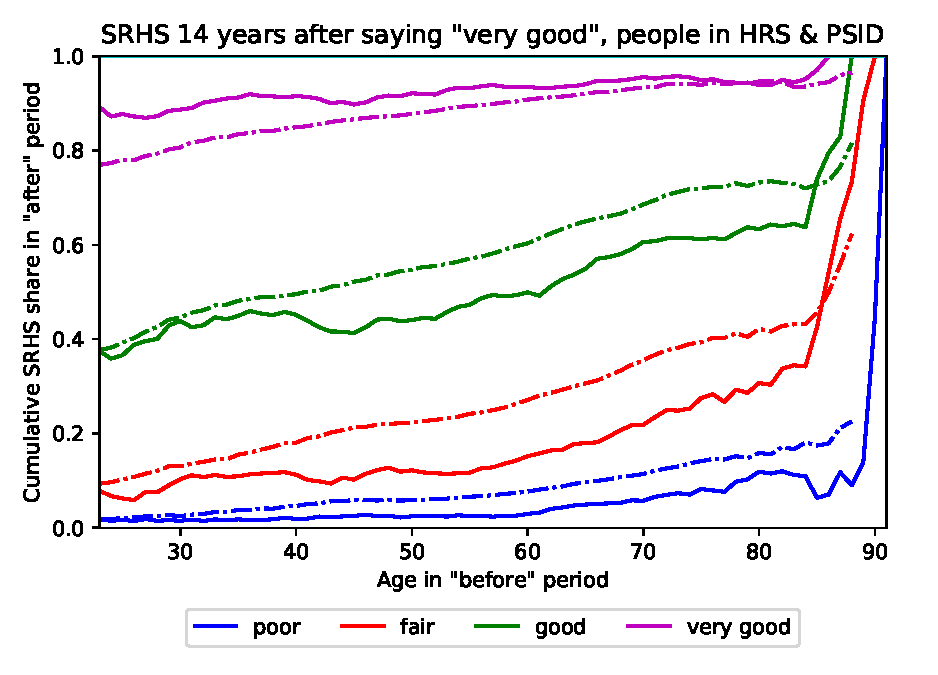
\includegraphics[width=\textwidth]{\FigsDir/TwoStudyOver23AllTransH4T14naive.pdf}
		\caption{Seven waves ahead}\label{fig:Naive7AheadVeryGood}
	\end{subfigure}
	~
	\begin{subfigure}[b]{0.48\textwidth}
		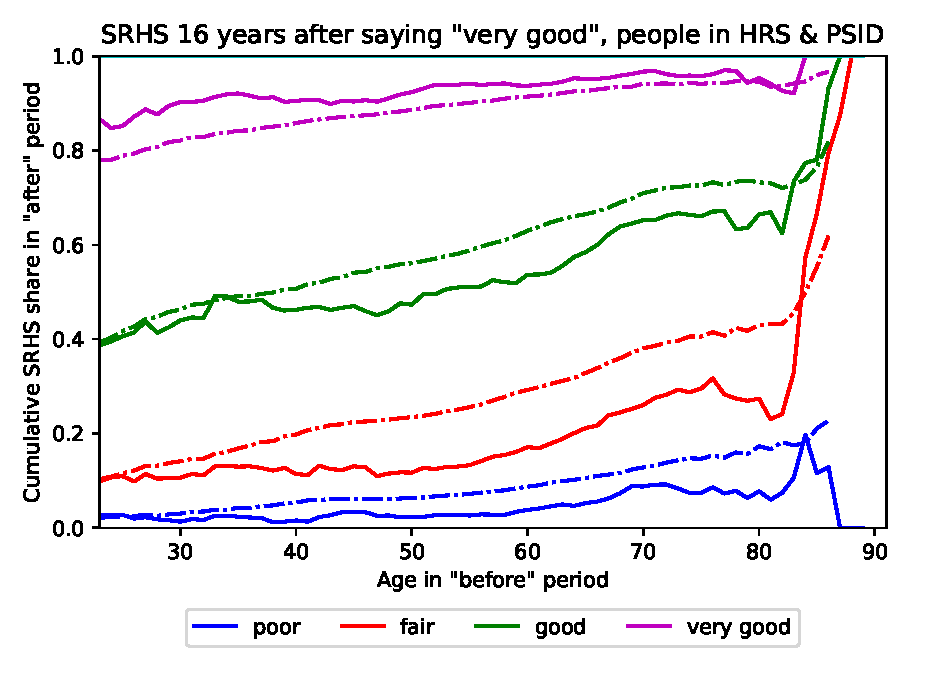
\includegraphics[width=\textwidth]{\FigsDir/TwoStudyOver23AllTransH4T16naive.pdf}
		\caption{Eight waves ahead}\label{fig:Naive8AheadVeryGood}
	\end{subfigure}
	\caption{Cumulative distribution of SRHS by age conditional on reporting ``very good'' health in the baseline period in the PSID \& HRS data (solid) vs simple dynamics (dash-dot).}\label{fig:NaiveTransVGa}
\end{figure}


\begin{figure}
	\centering
	\begin{subfigure}[b]{0.48\textwidth}
		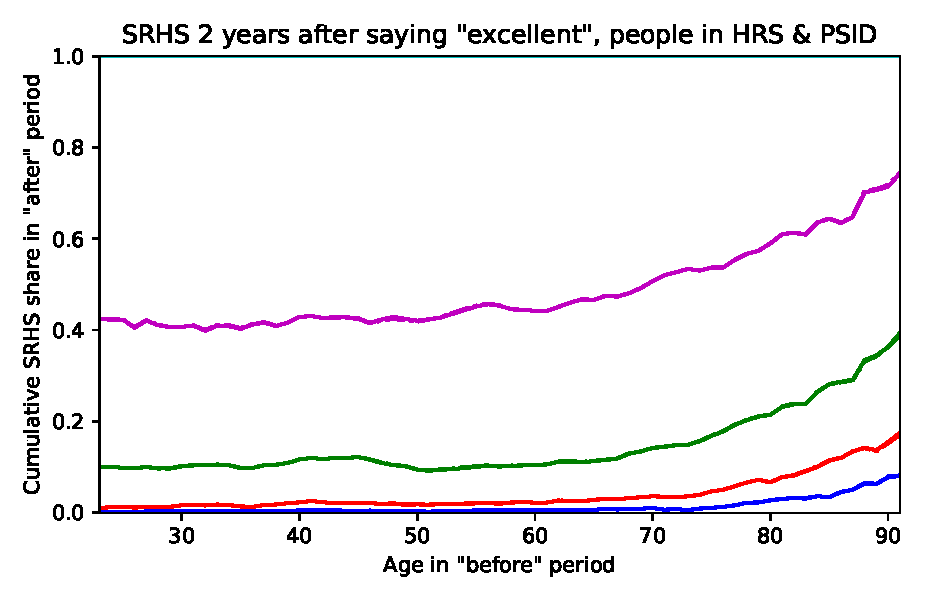
\includegraphics[width=\textwidth]{\FigsDir/TwoStudyOver23AllTransH5T2naiveNoLeg.pdf}
		\caption{One wave ahead}\label{fig:Naive1AheadExcellent}
	\end{subfigure}
	~
	\begin{subfigure}[b]{0.48\textwidth}
		\includegraphics[width=\textwidth]{\FigsDir/TwoStudyOver23AllTransH5T4naiveNoLeg.pdf}
		\caption{Two waves ahead}\label{fig:Naive2AheadExcellent}
	\end{subfigure}
	
	\begin{subfigure}[b]{0.48\textwidth}
		\includegraphics[width=\textwidth]{\FigsDir/TwoStudyOver23AllTransH5T6naiveNoLeg.pdf}
		\caption{Three waves ahead}\label{fig:Naive3AheadExcellent}
	\end{subfigure}
	~
	\begin{subfigure}[b]{0.48\textwidth}
		\includegraphics[width=\textwidth]{\FigsDir/TwoStudyOver23AllTransH5T8naiveNoLeg.pdf}
		\caption{Four waves ahead}\label{fig:Naive4AheadExcellent}
	\end{subfigure}
	
	\begin{subfigure}[b]{0.48\textwidth}
		\includegraphics[width=\textwidth]{\FigsDir/TwoStudyOver23AllTransH5T10naiveNoLeg.pdf}
		\caption{Five waves ahead}\label{fig:Naive5AheadExcellent}
	\end{subfigure}
	~
	\begin{subfigure}[b]{0.48\textwidth}
		\includegraphics[width=\textwidth]{\FigsDir/TwoStudyOver23AllTransH5T12naiveNoLeg.pdf}
		\caption{Six waves ahead}\label{fig:Naive6AheadExcellent}
	\end{subfigure}
	
	\begin{subfigure}[b]{0.48\textwidth}
		\includegraphics[width=\textwidth]{\FigsDir/TwoStudyOver23AllTransH5T14naive.pdf}
		\caption{Seven waves ahead}\label{fig:Naive7AheadExcellent}
	\end{subfigure}
	~
	\begin{subfigure}[b]{0.48\textwidth}
		\includegraphics[width=\textwidth]{\FigsDir/TwoStudyOver23AllTransH5T16naive.pdf}
		\caption{Eight waves ahead}\label{fig:Naive8AheadExcellent}
	\end{subfigure}
	\caption{Cumulative distribution of SRHS by age conditional on reporting ``excellent'' health in the baseline period in the PSID \& HRS data (solid) vs simple (dash-dot).}\label{fig:NaiveTransEX}
\end{figure}


\begin{figure}
	\centering
	\begin{subfigure}[b]{0.48\textwidth}
		\includegraphics[width=\textwidth]{\FigsDir/TwoStudyOver23AllTransH1T2modelNoLeg.pdf}
		\caption{One wave ahead}\label{fig:Model1AheadPoor}
	\end{subfigure}
	~
	\begin{subfigure}[b]{0.48\textwidth}
		\includegraphics[width=\textwidth]{\FigsDir/TwoStudyOver23AllTransH1T4modelNoLeg.pdf}
		\caption{Two waves ahead}\label{fig:Model2AheadPoor}
	\end{subfigure}
	
	\begin{subfigure}[b]{0.48\textwidth}
		\includegraphics[width=\textwidth]{\FigsDir/TwoStudyOver23AllTransH1T6modelNoLeg.pdf}
		\caption{Three waves ahead}\label{fig:Model3AheadPoor}
	\end{subfigure}
	~
	\begin{subfigure}[b]{0.48\textwidth}
		\includegraphics[width=\textwidth]{\FigsDir/TwoStudyOver23AllTransH1T8modelNoLeg.pdf}
		\caption{Four waves ahead}\label{fig:Model4AheadPoor}
	\end{subfigure}
	
	\begin{subfigure}[b]{0.48\textwidth}
		\includegraphics[width=\textwidth]{\FigsDir/TwoStudyOver23AllTransH1T10modelNoLeg.pdf}
		\caption{Five waves ahead}\label{fig:Model5AheadPoor}
	\end{subfigure}
	~
	\begin{subfigure}[b]{0.48\textwidth}
		\includegraphics[width=\textwidth]{\FigsDir/TwoStudyOver23AllTransH1T12modelNoLeg.pdf}
		\caption{Six waves ahead}\label{fig:Model6AheadPoor}
	\end{subfigure}

	\begin{subfigure}[b]{0.48\textwidth}
		\includegraphics[width=\textwidth]{\FigsDir/TwoStudyOver23AllTransH1T14model.pdf}
		\caption{Seven waves ahead}\label{fig:Model7AheadPoor}
	\end{subfigure}
	~
	\begin{subfigure}[b]{0.48\textwidth}
		\includegraphics[width=\textwidth]{\FigsDir/TwoStudyOver23AllTransH1T16model.pdf}
		\caption{Eight waves ahead}\label{fig:Model8AheadPoor}
	\end{subfigure}
	\caption{Cumulative distribution of SRHS by age conditional on reporting ``poor'' health in the baseline period in the PSID \& HRS data (solid) vs estimated model (dashed).}\label{fig:ModelTransPR}
\end{figure}


\begin{figure}
	\centering
	\begin{subfigure}[b]{0.48\textwidth}
		\includegraphics[width=\textwidth]{\FigsDir/TwoStudyOver23AllTransH2T2modelNoLeg.pdf}
		\caption{One wave ahead}\label{fig:Model1AheadFair}
	\end{subfigure}
	~
	\begin{subfigure}[b]{0.48\textwidth}
		\includegraphics[width=\textwidth]{\FigsDir/TwoStudyOver23AllTransH2T4modelNoLeg.pdf}
		\caption{Two waves ahead}\label{fig:Model2AheadFair}
	\end{subfigure}
	
	\begin{subfigure}[b]{0.48\textwidth}
		\includegraphics[width=\textwidth]{\FigsDir/TwoStudyOver23AllTransH2T6modelNoLeg.pdf}
		\caption{Three waves ahead}\label{fig:Model3AheadFair}
	\end{subfigure}
	~
	\begin{subfigure}[b]{0.48\textwidth}
		\includegraphics[width=\textwidth]{\FigsDir/TwoStudyOver23AllTransH2T8modelNoLeg.pdf}
		\caption{Four waves ahead}\label{fig:Model4AheadFair}
	\end{subfigure}
	
	\begin{subfigure}[b]{0.48\textwidth}
		\includegraphics[width=\textwidth]{\FigsDir/TwoStudyOver23AllTransH2T10modelNoLeg.pdf}
		\caption{Five waves ahead}\label{fig:Model5AheadFair}
	\end{subfigure}
	~
	\begin{subfigure}[b]{0.48\textwidth}
		\includegraphics[width=\textwidth]{\FigsDir/TwoStudyOver23AllTransH2T12modelNoLeg.pdf}
		\caption{Six waves ahead}\label{fig:Model6AheadFair}
	\end{subfigure}

	\begin{subfigure}[b]{0.48\textwidth}
		\includegraphics[width=\textwidth]{\FigsDir/TwoStudyOver23AllTransH2T14model.pdf}
		\caption{Seven waves ahead}\label{fig:Model7AheadFair}
	\end{subfigure}
	~
	\begin{subfigure}[b]{0.48\textwidth}
		\includegraphics[width=\textwidth]{\FigsDir/TwoStudyOver23AllTransH2T16model.pdf}
		\caption{Eight waves ahead}\label{fig:Model8AheadFair}
	\end{subfigure}
	\caption{Cumulative distribution of SRHS by age conditional on reporting ``fair'' health in the baseline period in the PSID \& HRS data (solid) vs estimated model (dashed).}\label{fig:ModelTransFR}
\end{figure}


\begin{figure}
	\centering
	\begin{subfigure}[b]{0.48\textwidth}
		\includegraphics[width=\textwidth]{\FigsDir/TwoStudyOver23AllTransH3T2modelNoLeg.pdf}
		\caption{One wave ahead}\label{fig:Model1AheadGood}
	\end{subfigure}
	~
	\begin{subfigure}[b]{0.48\textwidth}
		\includegraphics[width=\textwidth]{\FigsDir/TwoStudyOver23AllTransH3T4modelNoLeg.pdf}
		\caption{Two waves ahead}\label{fig:Model2AheadGood}
	\end{subfigure}
	
	\begin{subfigure}[b]{0.48\textwidth}
		\includegraphics[width=\textwidth]{\FigsDir/TwoStudyOver23AllTransH3T6modelNoLeg.pdf}
		\caption{Three waves ahead}\label{fig:Model3AheadGood}
	\end{subfigure}
	~
	\begin{subfigure}[b]{0.48\textwidth}
		\includegraphics[width=\textwidth]{\FigsDir/TwoStudyOver23AllTransH3T8modelNoLeg.pdf}
		\caption{Four waves ahead}\label{fig:Model4AheadGood}
	\end{subfigure}
	
	\begin{subfigure}[b]{0.48\textwidth}
		\includegraphics[width=\textwidth]{\FigsDir/TwoStudyOver23AllTransH3T10modelNoLeg.pdf}
		\caption{Five waves ahead}\label{fig:Model5AheadGood}
	\end{subfigure}
	~
	\begin{subfigure}[b]{0.48\textwidth}
		\includegraphics[width=\textwidth]{\FigsDir/TwoStudyOver23AllTransH3T12modelNoLeg.pdf}
		\caption{Six waves ahead}\label{fig:Model6AheadGood}
	\end{subfigure}
	
	\begin{subfigure}[b]{0.48\textwidth}
		\includegraphics[width=\textwidth]{\FigsDir/TwoStudyOver23AllTransH3T14model.pdf}
		\caption{Seven waves ahead}\label{fig:Model7AheadGood}
	\end{subfigure}
	~
	\begin{subfigure}[b]{0.48\textwidth}
		\includegraphics[width=\textwidth]{\FigsDir/TwoStudyOver23AllTransH3T16model.pdf}
		\caption{Eight waves ahead}\label{fig:Model8AheadGood}
	\end{subfigure}
	\caption{Cumulative distribution of SRHS by age conditional on reporting ``good'' health in the baseline period in the PSID \& HRS data (solid) vs estimated model (dashed).}\label{fig:ModelTransGD}
\end{figure}


\begin{figure}
	\centering
	\begin{subfigure}[b]{0.48\textwidth}
		\includegraphics[width=\textwidth]{\FigsDir/TwoStudyOver23AllTransH4T2modelNoLeg.pdf}
		\caption{One wave ahead}\label{fig:Model1AheadVeryGood}
	\end{subfigure}
	~
	\begin{subfigure}[b]{0.48\textwidth}
		\includegraphics[width=\textwidth]{\FigsDir/TwoStudyOver23AllTransH4T4modelNoLeg.pdf}
		\caption{Two waves ahead}\label{fig:Model2AheadVeryGood}
	\end{subfigure}
	
	\begin{subfigure}[b]{0.48\textwidth}
		\includegraphics[width=\textwidth]{\FigsDir/TwoStudyOver23AllTransH4T6modelNoLeg.pdf}
		\caption{Three waves ahead}\label{fig:Model3AheadVeryGood}
	\end{subfigure}
	~
	\begin{subfigure}[b]{0.48\textwidth}
		\includegraphics[width=\textwidth]{\FigsDir/TwoStudyOver23AllTransH4T8modelNoLeg.pdf}
		\caption{Four waves ahead}\label{fig:Model4AheadVeryGood}
	\end{subfigure}
	
	\begin{subfigure}[b]{0.48\textwidth}
		\includegraphics[width=\textwidth]{\FigsDir/TwoStudyOver23AllTransH4T10modelNoLeg.pdf}
		\caption{Five waves ahead}\label{fig:Model5AheadVeryGood}
	\end{subfigure}
	~
	\begin{subfigure}[b]{0.48\textwidth}
		\includegraphics[width=\textwidth]{\FigsDir/TwoStudyOver23AllTransH4T12modelNoLeg.pdf}
		\caption{Six waves ahead}\label{fig:Model6AheadVeryGood}
	\end{subfigure}
	
	\begin{subfigure}[b]{0.48\textwidth}
		\includegraphics[width=\textwidth]{\FigsDir/TwoStudyOver23AllTransH4T14model.pdf}
		\caption{Seven waves ahead}\label{fig:Model7AheadVeryGood}
	\end{subfigure}
	~
	\begin{subfigure}[b]{0.48\textwidth}
		\includegraphics[width=\textwidth]{\FigsDir/TwoStudyOver23AllTransH4T16model.pdf}
		\caption{Eight waves ahead}\label{fig:Model8AheadVeryGood}
	\end{subfigure}
	\caption{Cumulative distribution of SRHS by age conditional on reporting ``very good'' health in the baseline period in the PSID \& HRS data (solid) vs estimated model (dashed).}\label{fig:ModelTransVGa}
\end{figure}


\begin{figure}
	\centering
	\begin{subfigure}[b]{0.48\textwidth}
		\includegraphics[width=\textwidth]{\FigsDir/TwoStudyOver23AllTransH5T2modelNoLeg.pdf}
		\caption{One wave ahead}\label{fig:Model1AheadExcellent}
	\end{subfigure}
	~
	\begin{subfigure}[b]{0.48\textwidth}
		\includegraphics[width=\textwidth]{\FigsDir/TwoStudyOver23AllTransH5T4modelNoLeg.pdf}
		\caption{Two waves ahead}\label{fig:Model2AheadExcellent}
	\end{subfigure}
	
	\begin{subfigure}[b]{0.48\textwidth}
		\includegraphics[width=\textwidth]{\FigsDir/TwoStudyOver23AllTransH5T6modelNoLeg.pdf}
		\caption{Three waves ahead}\label{fig:Model3AheadExcellent}
	\end{subfigure}
	~
	\begin{subfigure}[b]{0.48\textwidth}
		\includegraphics[width=\textwidth]{\FigsDir/TwoStudyOver23AllTransH5T8modelNoLeg.pdf}
		\caption{Four waves ahead}\label{fig:Model4AheadExcellent}
	\end{subfigure}
	
	\begin{subfigure}[b]{0.48\textwidth}
		\includegraphics[width=\textwidth]{\FigsDir/TwoStudyOver23AllTransH5T10modelNoLeg.pdf}
		\caption{Five waves ahead}\label{fig:Model5AheadExcellent}
	\end{subfigure}
	~
	\begin{subfigure}[b]{0.48\textwidth}
		\includegraphics[width=\textwidth]{\FigsDir/TwoStudyOver23AllTransH5T12modelNoLeg.pdf}
		\caption{Six waves ahead}\label{fig:Model6AheadExcellent}
	\end{subfigure}
	
	\begin{subfigure}[b]{0.48\textwidth}
		\includegraphics[width=\textwidth]{\FigsDir/TwoStudyOver23AllTransH5T14model.pdf}
		\caption{Seven waves ahead}\label{fig:Model7AheadExcellent}
	\end{subfigure}
	~
	\begin{subfigure}[b]{0.48\textwidth}
		\includegraphics[width=\textwidth]{\FigsDir/TwoStudyOver23AllTransH5T16model.pdf}
		\caption{Eight waves ahead}\label{fig:Model8AheadExcellent}
	\end{subfigure}
	\caption{Cumulative distribution of SRHS by age conditional on reporting ``excellent'' health in the baseline period in the PSID \& HRS data (solid) vs estimated model (dashed).}\label{fig:ModelTransEX}
\end{figure}


\begin{figure}
	\centering
	\begin{subfigure}[b]{0.48\textwidth}
		\includegraphics[width=\textwidth]{\FigsDir/TwoStudyOver23AllSRHSfreqH25to34.pdf}
		\caption{``Healthy'' aged 25-34 at baseline}\label{fig:SRHSfreqH25to34}
	\end{subfigure}
	~
	\begin{subfigure}[b]{0.48\textwidth}
		\includegraphics[width=\textwidth]{\FigsDir/TwoStudyOver23AllSRHSfreqH35to44.pdf}
		\caption{``Healthy'' aged 35-44 at baseline}\label{fig:SRHSfreqH35to44}
	\end{subfigure}
	
	\begin{subfigure}[b]{0.48\textwidth}
		\includegraphics[width=\textwidth]{\FigsDir/TwoStudyOver23AllSRHSfreqH45to54.pdf}
		\caption{``Healthy'' aged 45-54 at baseline}\label{fig:SRHSfreqH45to54}
	\end{subfigure}
	~
	\begin{subfigure}[b]{0.48\textwidth}
		\includegraphics[width=\textwidth]{\FigsDir/TwoStudyOver23AllSRHSfreqH55to64.pdf}
		\caption{``Healthy'' aged 55-64 at baseline}\label{fig:SRHSfreqH55to64}
	\end{subfigure}
	
	
	\begin{subfigure}[b]{0.48\textwidth}
		\includegraphics[width=\textwidth]{\FigsDir/TwoStudyOver23AllSRHSfreqH65to74.pdf}
		\caption{``Healthy'' aged 65-74 at baseline}\label{fig:SRHSfreqH65to74}
	\end{subfigure}
	~
	\begin{subfigure}[b]{0.48\textwidth}
		\includegraphics[width=\textwidth]{\FigsDir/TwoStudyOver23AllSRHSfreqH75to84.pdf}
		\caption{``Healthy'' aged 75-84 at baseline}\label{fig:SRHSfreqH75to84}
	\end{subfigure}
	\caption{Distribution of number of times reporting unhealthy SRHS by age and health over next six waves conditional on being healthy at baseline, data vs estimated model vs simple dynamics. Relative to usual assumptions, the latent health model better matches the fraction of respondents who never report bad health.}\label{fig:SRHSfreqHTwoStudy}
\end{figure}

\begin{figure}
	\centering
	\includegraphics[scale=0.7]{\FigsDir/TwoStudyOver23AllChangeSRHS.pdf}
	\caption{Predicted probability of changing SRHS if asked twice in same survey. Dashed black line represents population average.}\label{fig:ChangeSRHS}
\end{figure}

\newpage

\bibliographystyle{mnwteststyle}
\bibliography{HiddenHealth}

\end{document}

